% ----------------------------------------------------------
% Apêndices
% Documentos gerados pelo próprio autor
% ----------------------------------------------------------

% ---
% Inicia os apêndices
% ---
\begin{apendicesenv}

% Imprime uma página indicando o início dos apêndices
\partapendices

\chapter{PROTOTIPAÇÃO}
\label{apendice_a}

\section{Tela Inicial do administrador}
\begin{figure}[H]
    \centering
    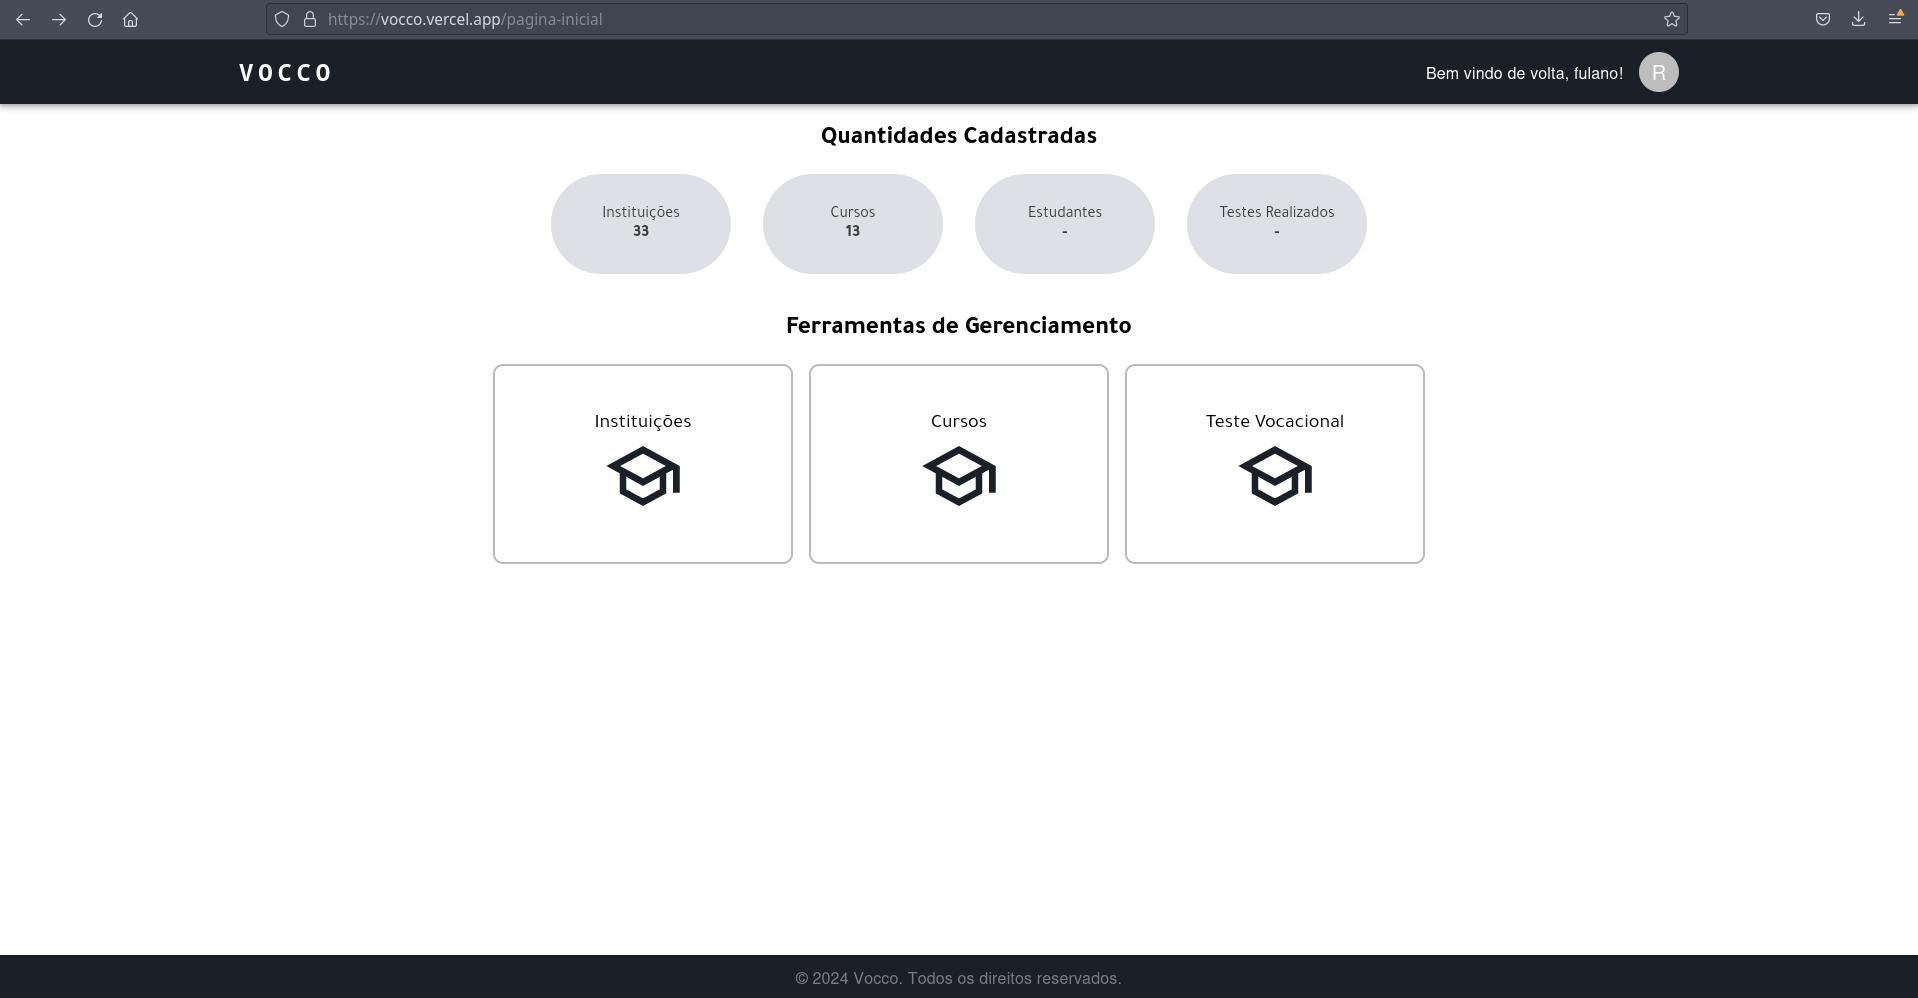
\includegraphics[width=1.0\linewidth]{images/telaInicial.png}
    \caption{Tela inicial do administrador}
    \label{fig:tela-inicial}
\end{figure}

\section{Tela de cadastro de dados gerais da instituição}
\begin{figure}[H]
    \centering
    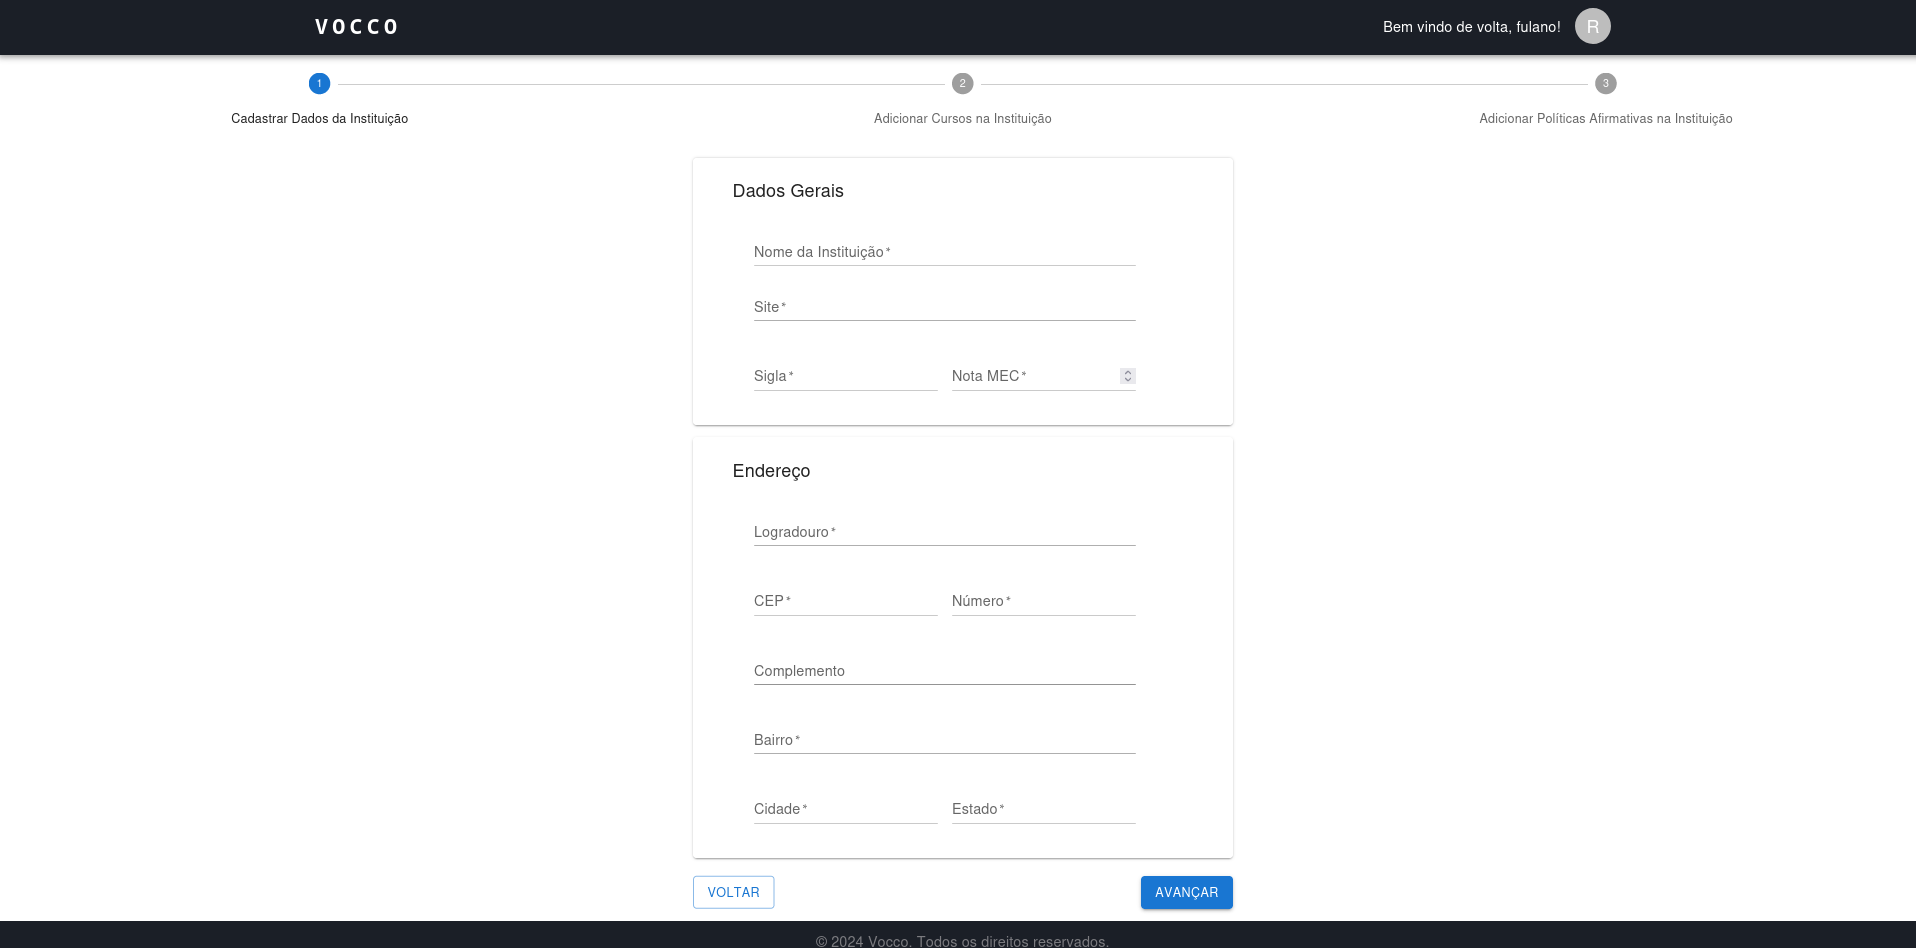
\includegraphics[width=1.0\linewidth]{images/dadosGerais.png}
    \caption{Cadastro de dados gerais da instituição}
    \label{fig:dados-gerais}
\end{figure}

\section{Tela de gerenciamento de instituições}
\begin{figure}[H]
    \centering
    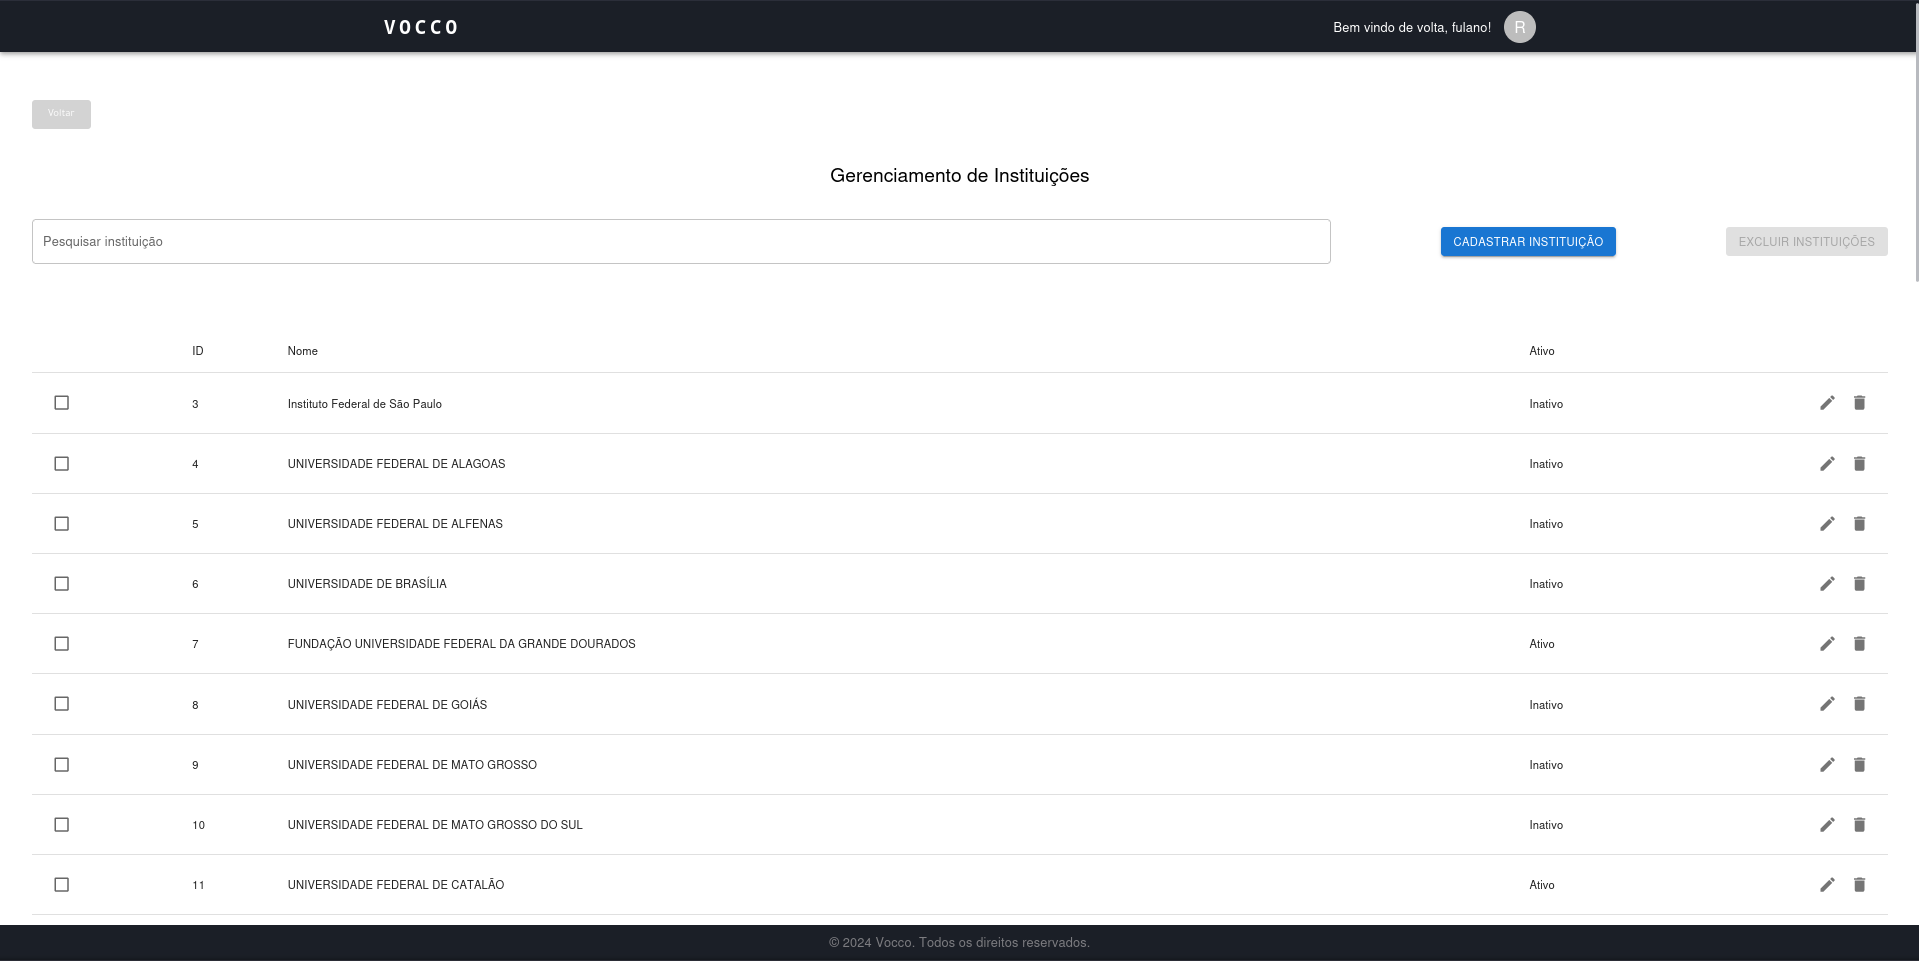
\includegraphics[width=1.0\linewidth]{images/gerenciamento.png}
    \caption{Gerenciamento de instituições}
    \label{fig:gerenciamento}
\end{figure}

\section{Tela de detalhamento de uma instituição}
\begin{figure}[H]
    \centering
    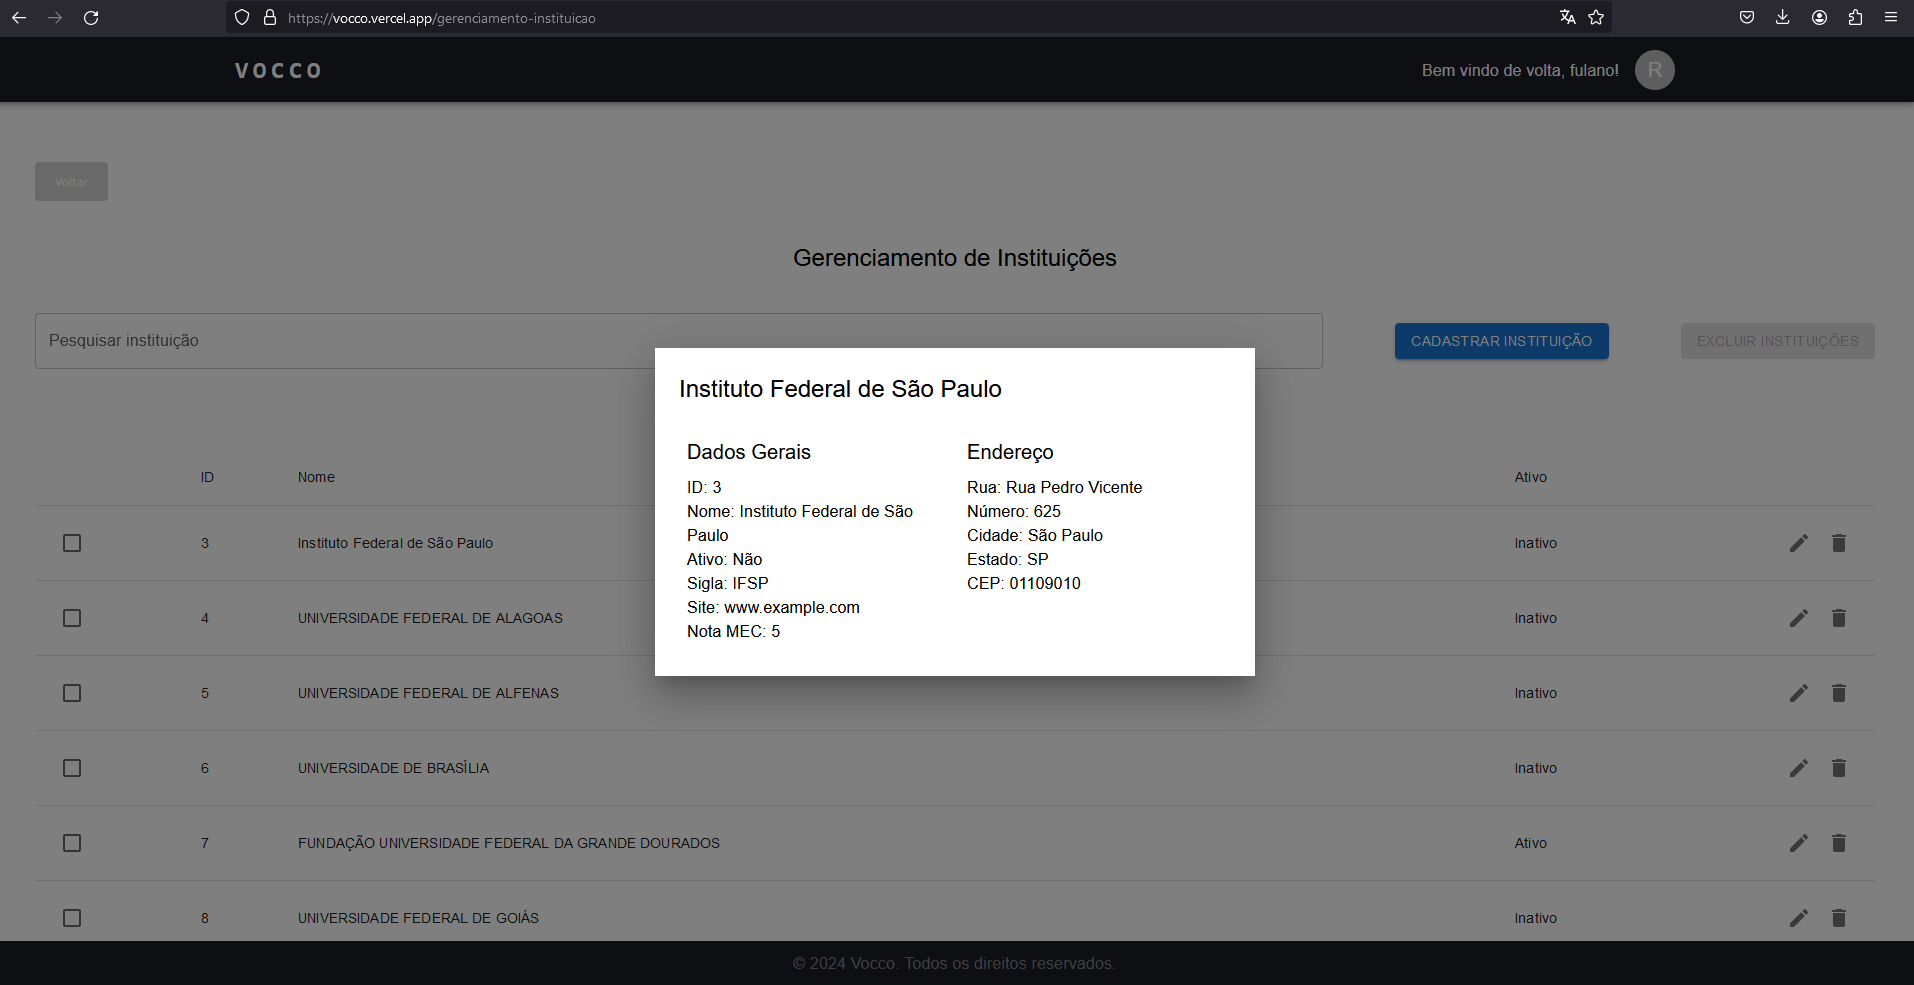
\includegraphics[width=1.0\linewidth]{images/informacoes.png}
    \caption{Cadastro de dados gerais da instituição}
    \label{fig:detalhamento}
\end{figure}

\section{Tela de edição de uma instituição}
\begin{figure}[H]
    \centering
    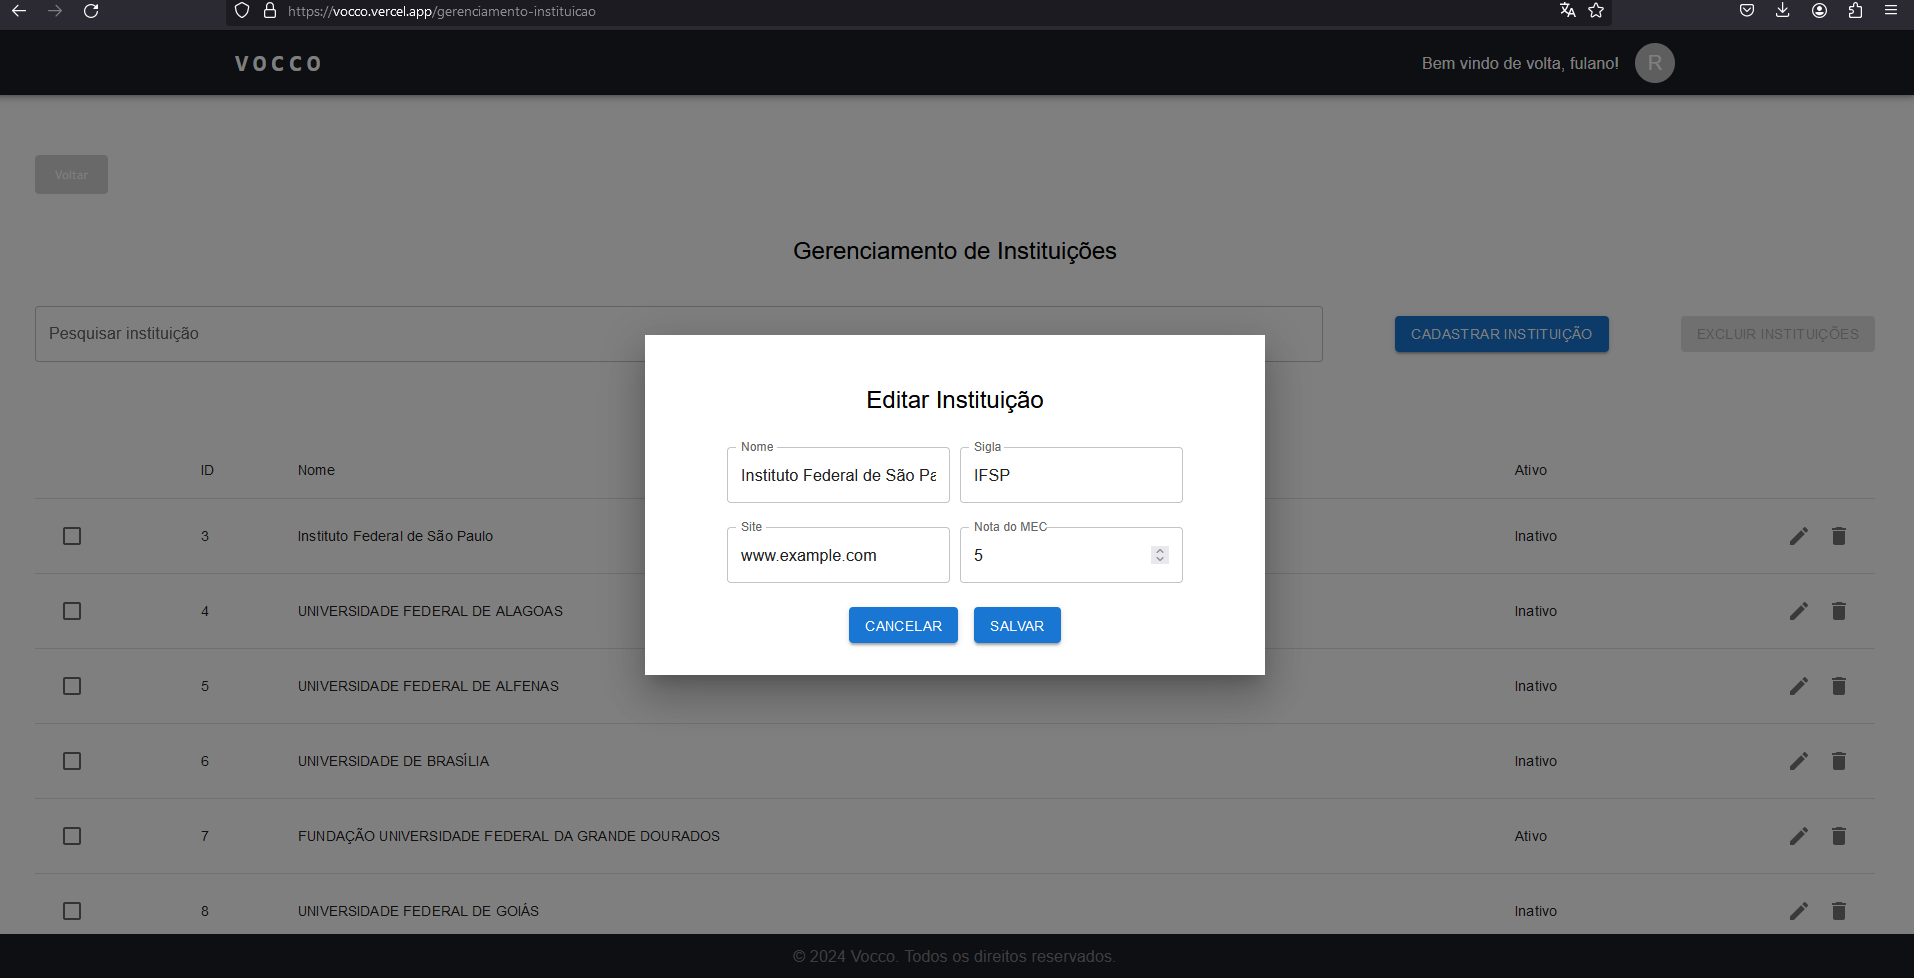
\includegraphics[width=1.0\linewidth]{images/editar.png}
    \caption{Cadastro de dados gerais da instituição}
    \label{fig:editar}
\end{figure}

\section{Tela de exclusão de uma instituição}
\begin{figure}[H]
    \centering
    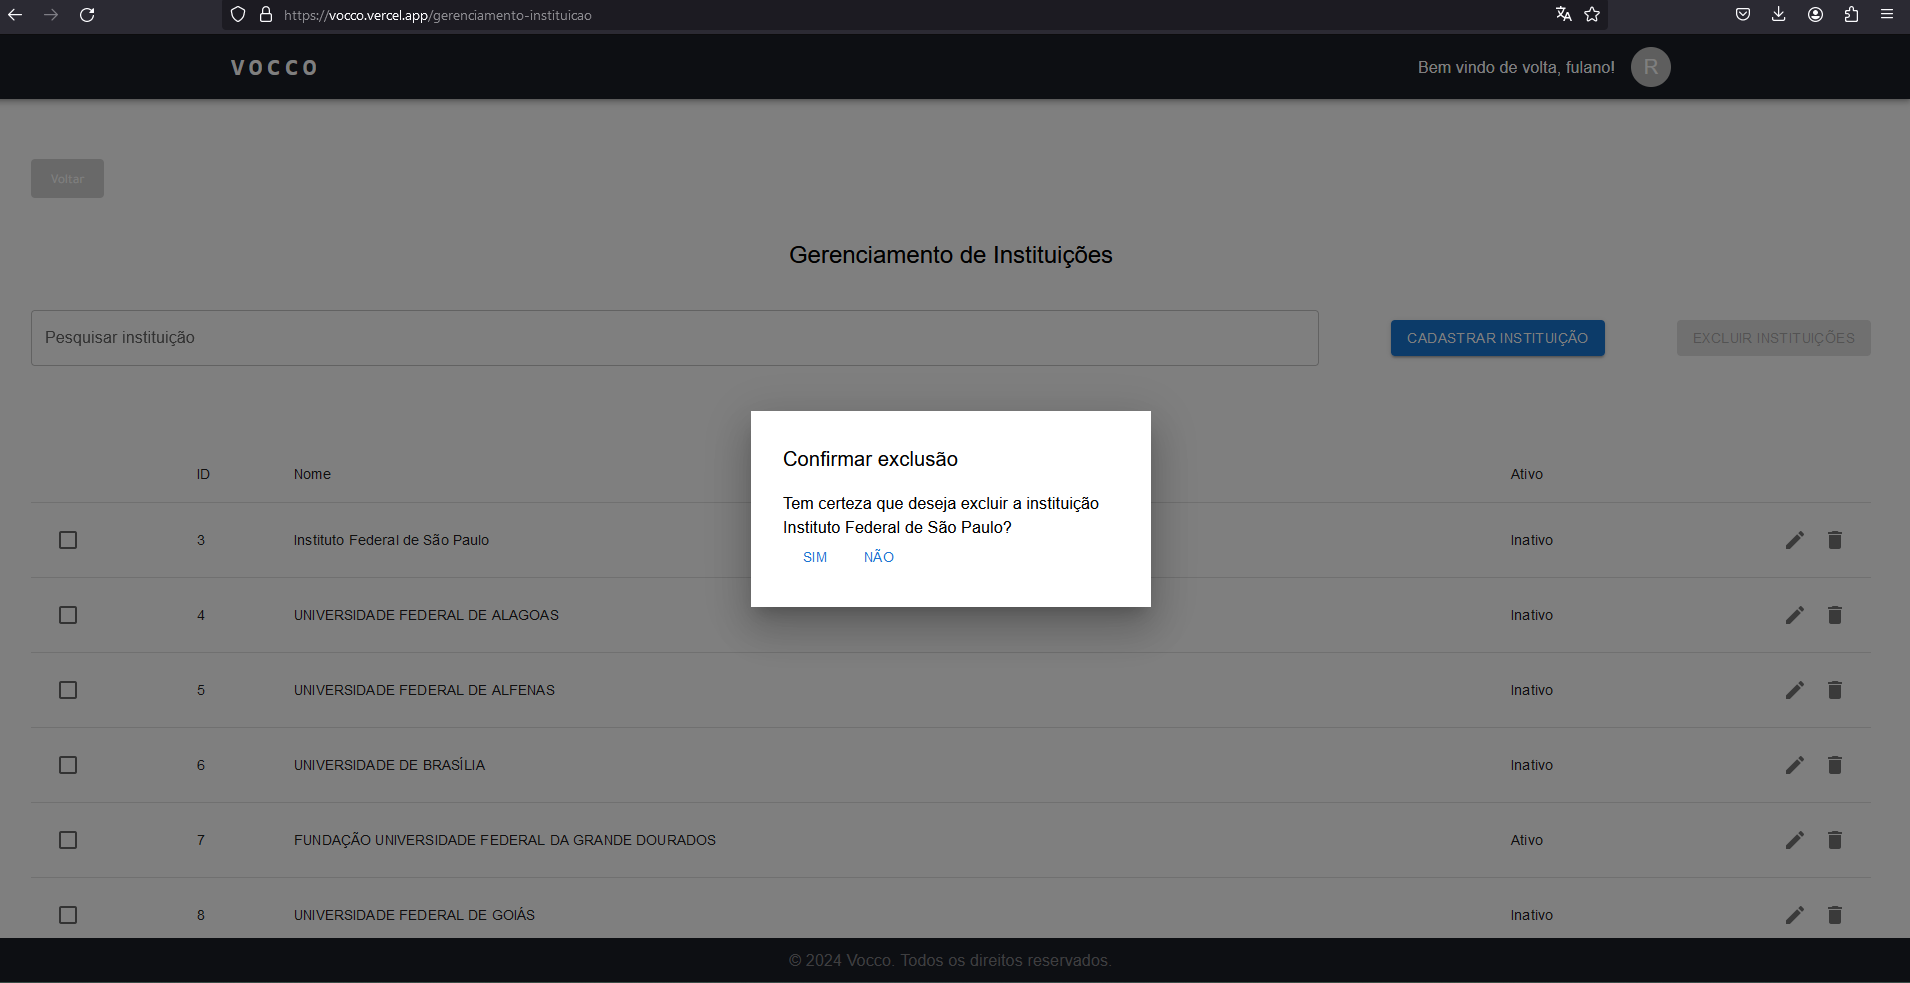
\includegraphics[width=1.0\linewidth]{images/exclusao.png}
    \caption{Cadastro de dados gerais da instituição}
    \label{fig:exclusao}
\end{figure}

\section{Tela de associação de instituições com cursos}
\begin{figure}[H]
    \centering
    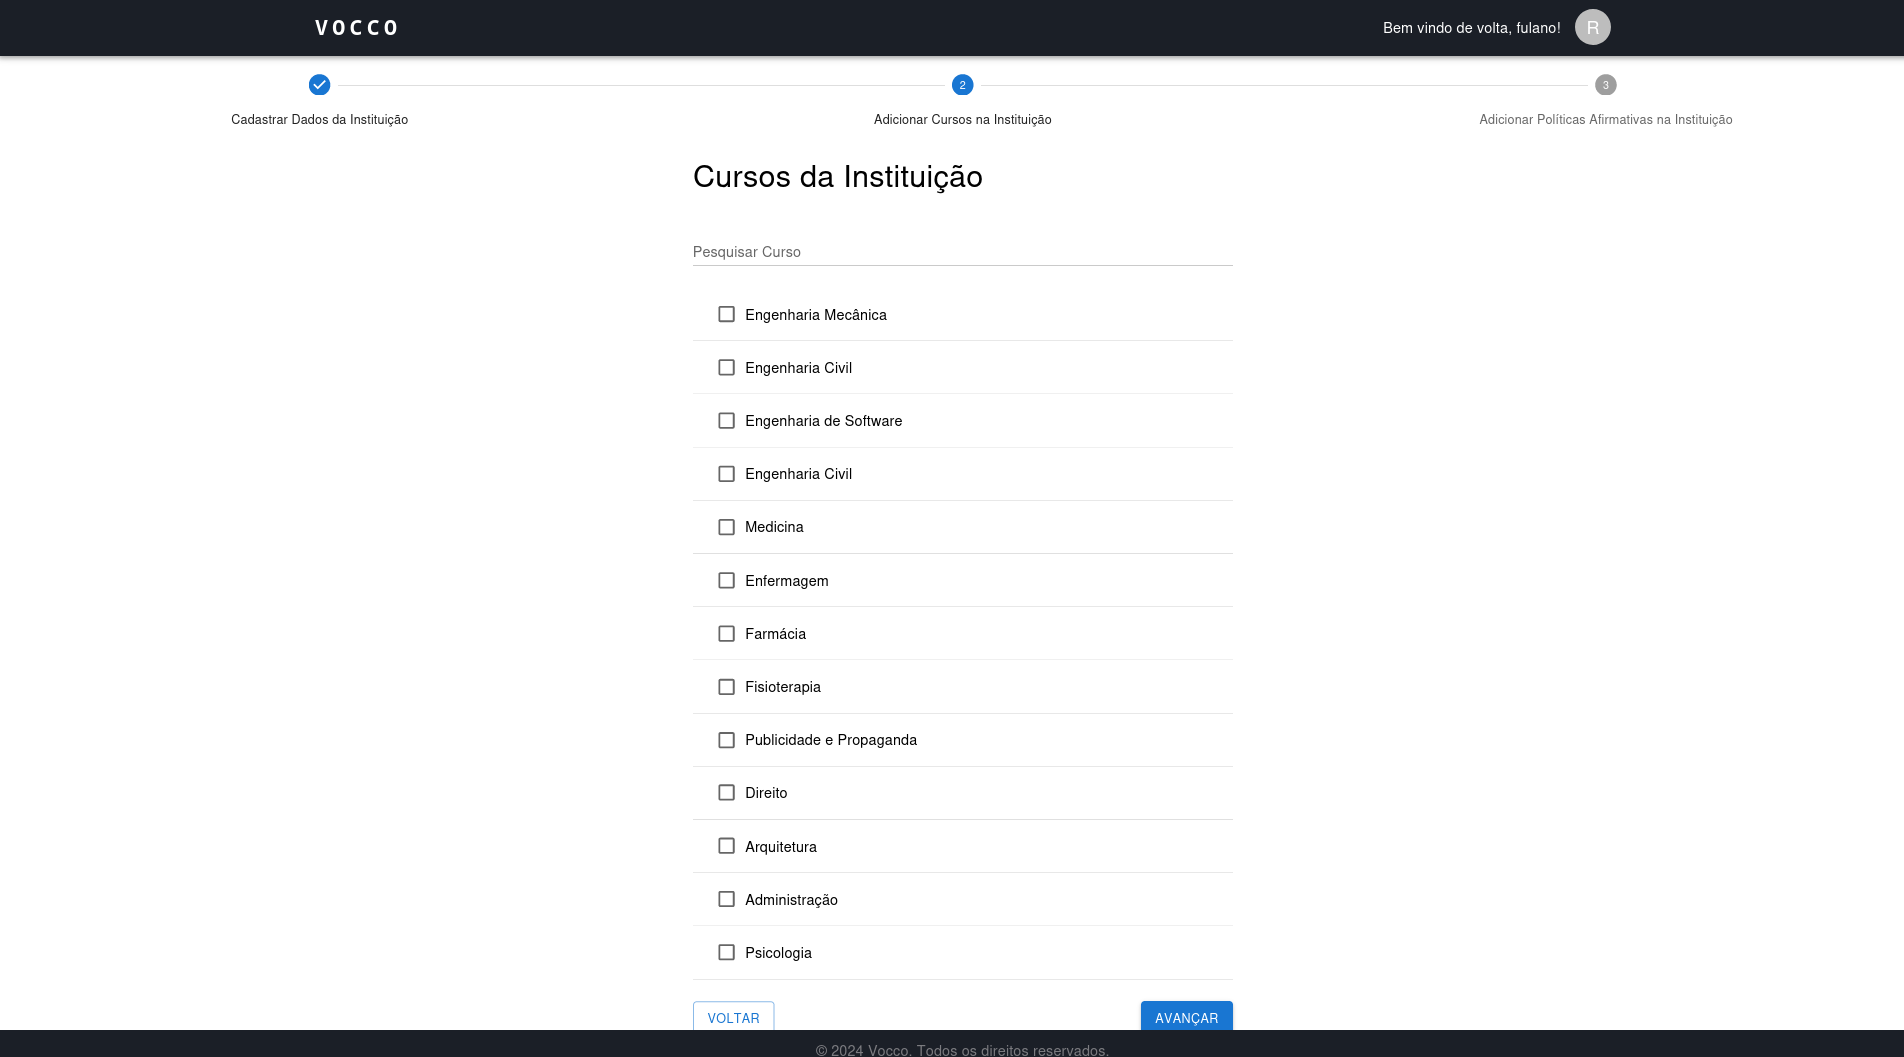
\includegraphics[width=1.0\linewidth]{images/cursos.png}
    \caption{Inserção dos cursos na instituição}
    \label{fig:cursos}
\end{figure}

\section{Tela de associação de instituições com políticas}
\begin{figure}[H]
    \centering
    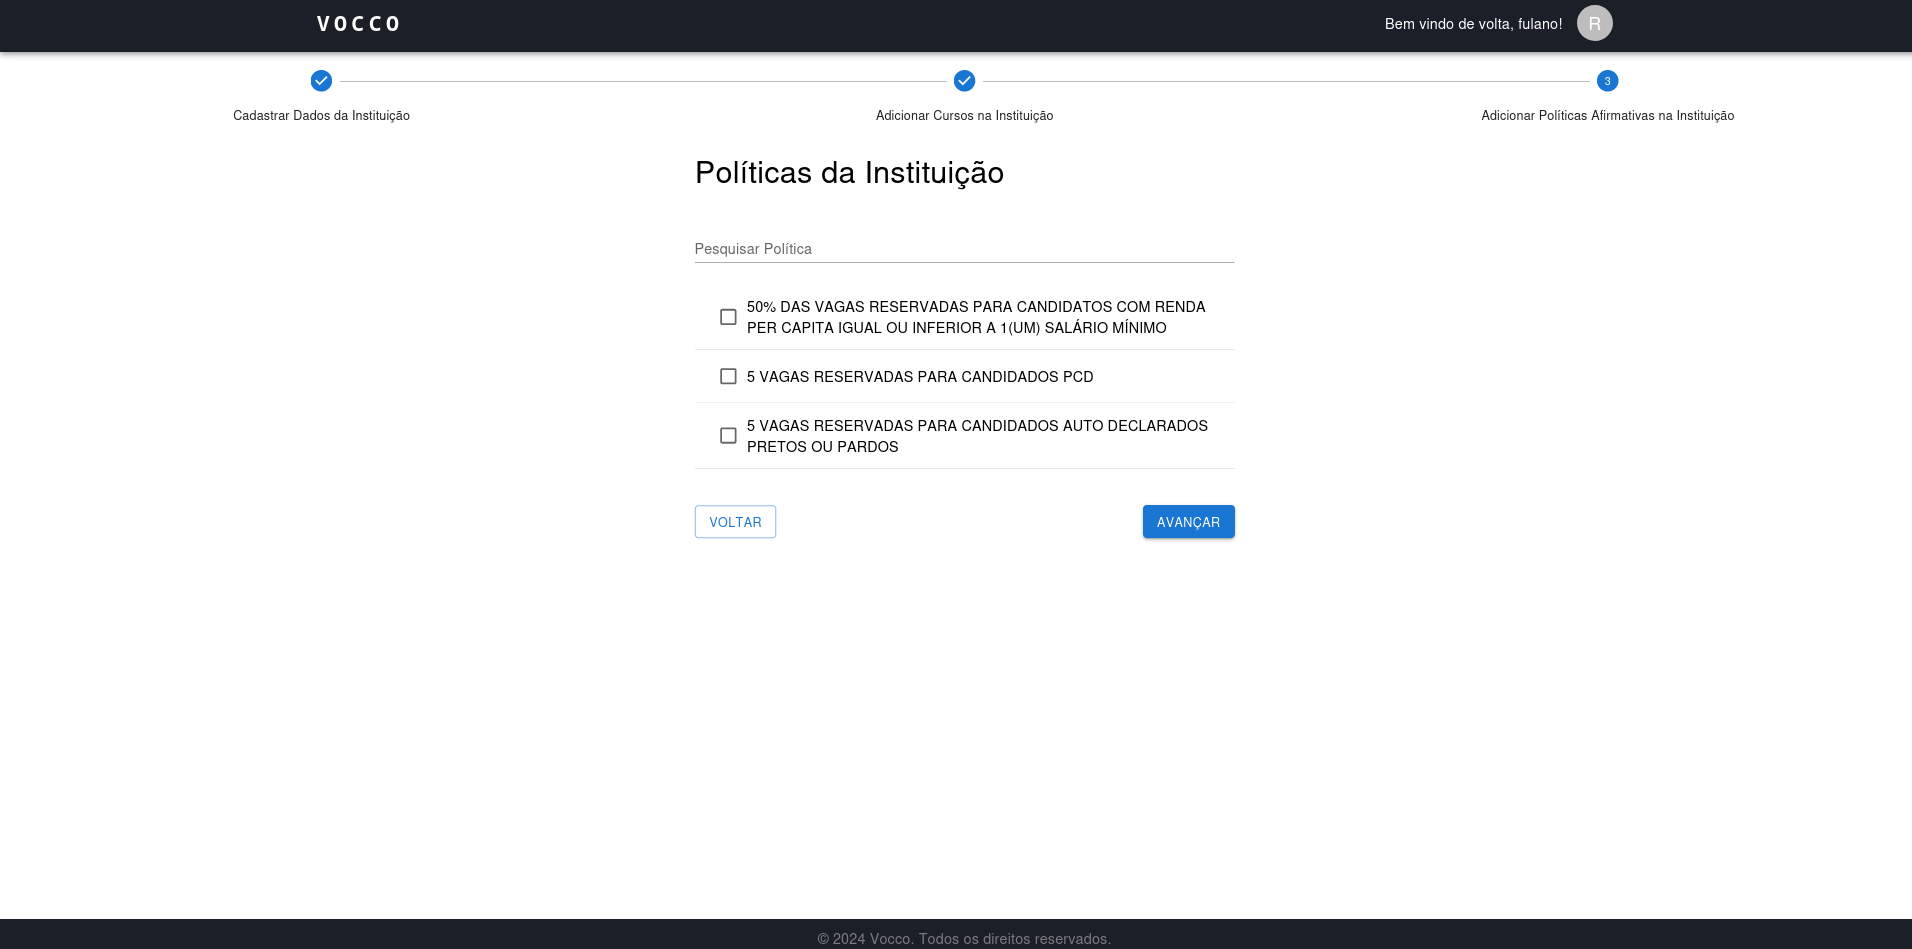
\includegraphics[width=1.0\linewidth]{images/politicas.png}
    \caption{Inserção das políticas na instituição}
    \label{fig:politicas}
\end{figure}

\chapter{Cronograma}
\label{apendice_i}
Para a organização e planejamento do desenvolvimento do projeto, dividimos as atribuições entre os integrantes do grupo. Dessa forma, conseguimos definir as datas de entrega e segui-las com mais facilidade. Com isso, o cronograma manteve um fluxo mais dinâmico e organizado, atendendo aos prazos estabelecidos para a entrega de cada fase do projeto.
\subsection*{Back-End}
Atividades e prazos definidos para o \textit{back-end} no decorrer do segundo semestre de 2024.

\begin{figure}[ht]
        \centering
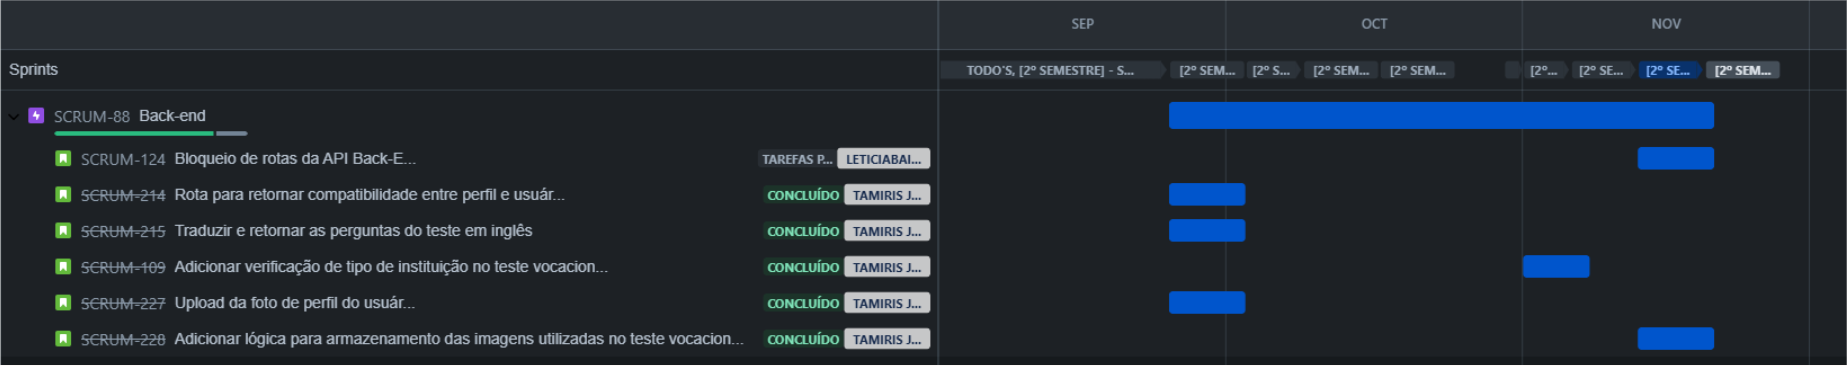
\includegraphics[width=1.0\textwidth]{images/back-end-cronograma.png}
        \caption{Cronograma definido para o \textit{back-end} no segundo semestre de 2024}
        \label{fig:backendcronograma}
    \end{figure}
As atividades do \textit{back-end} foram em sua maior parte concluídas no primeiro semestre de 2024, sendo que no segundo semestre foram feitos somentes ajustes necessários.    
\newpage
    
\subsection*{Base de Dados}
Atividades e prazos definidos para a realização de cadastros na base de dados no decorrer do segundo semestre de 2024. 

\begin{figure}[ht]
        \centering
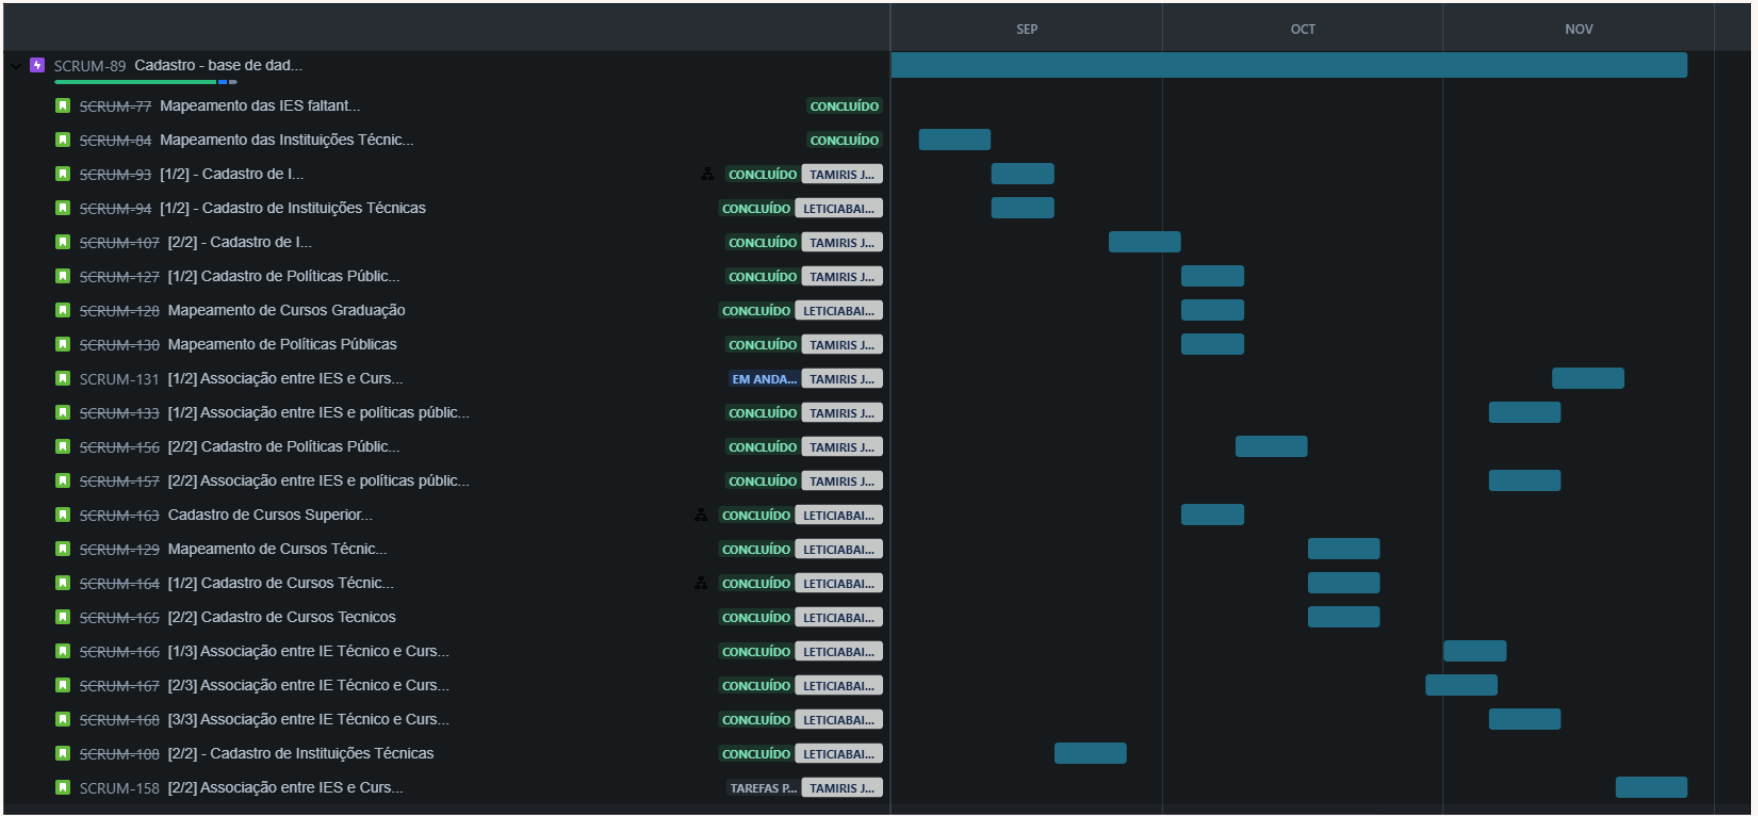
\includegraphics[width=1.0\textwidth]{images/base-dados-cronograma.png}
        \caption{Cronograma definido para os cadastros na base de dados no segundo semestre de 2024}
        \label{fig:basedadoscronograma}
    \end{figure}
As integrantes do grupo responsáveis pelo \textit{back-end} ficaram responsáveis pelos cadastros na base de dados no segundo semestre.

\subsection*{Design Visual}
Atividades e prazos definidos para a finalização do design visual do projeto no decorrer do segundo semestre de 2024. 

\begin{figure}[ht]
        \centering
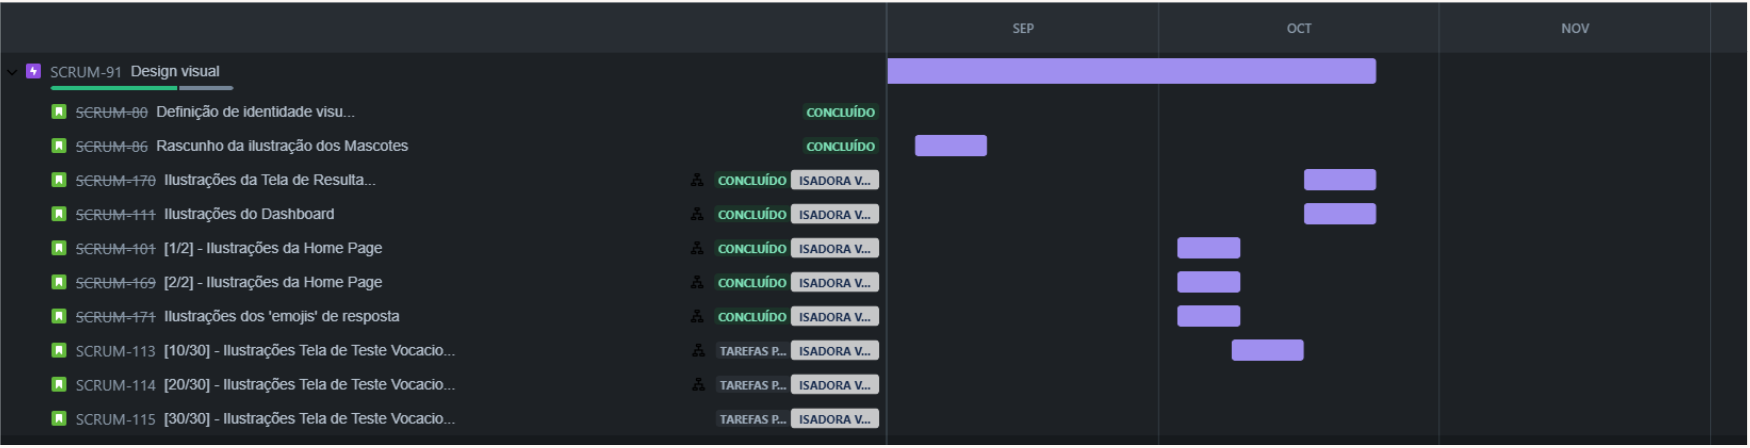
\includegraphics[width=1.0\textwidth]{images/design-visual-cronograma.png}
        \caption{Cronograma definido para o design visual no segundo semestre de 2024}
        \label{fig:designvisualcronograma}
    \end{figure}
\newpage

Com a refatoração da telas, se fez necessário novos designs visuais para o projeto.

\subsection*{Front-End}
Atividades e prazos definidos para o \textit{back-end} no decorrer do segundo semestre de 2024.

\begin{figure}[ht]
        \centering
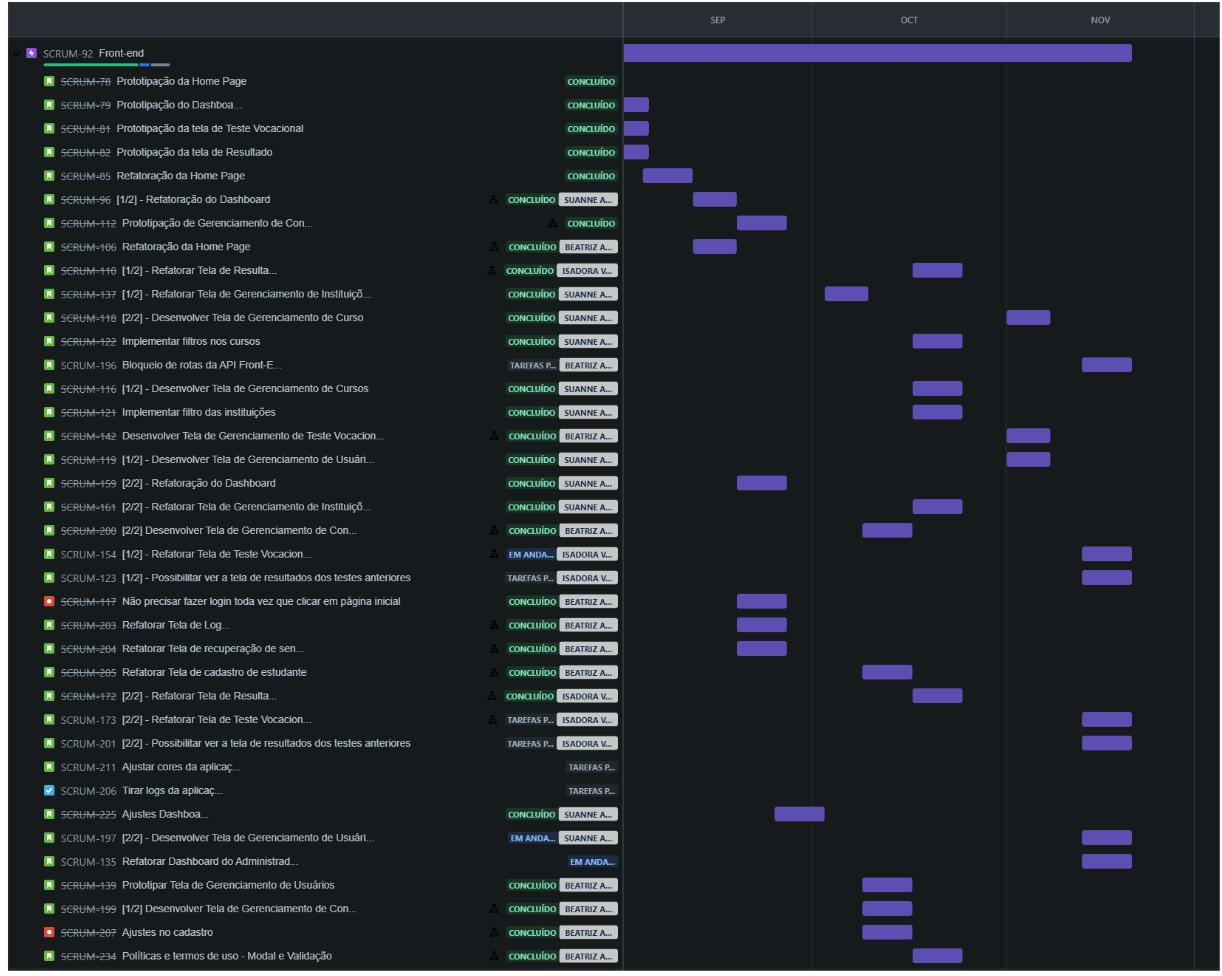
\includegraphics[width=1.0\textwidth]{images/front-end-cronograma.png}
        \caption{Cronograma definido para o \textit{front-end} no segundo semestre de 2024}
        \label{fig:frontendcronograma}
    \end{figure}
\newpage

Com a refatoração da telas, o front-end ficou com mais tarefas que o \textit{back-end}.

\subsection*{Revisões e Documentação}
Atividades e prazos definidos para finalizar as tarefa de revisão e documentação no decorrer do segundo semestre de 2024.

\begin{figure}[ht]
        \centering
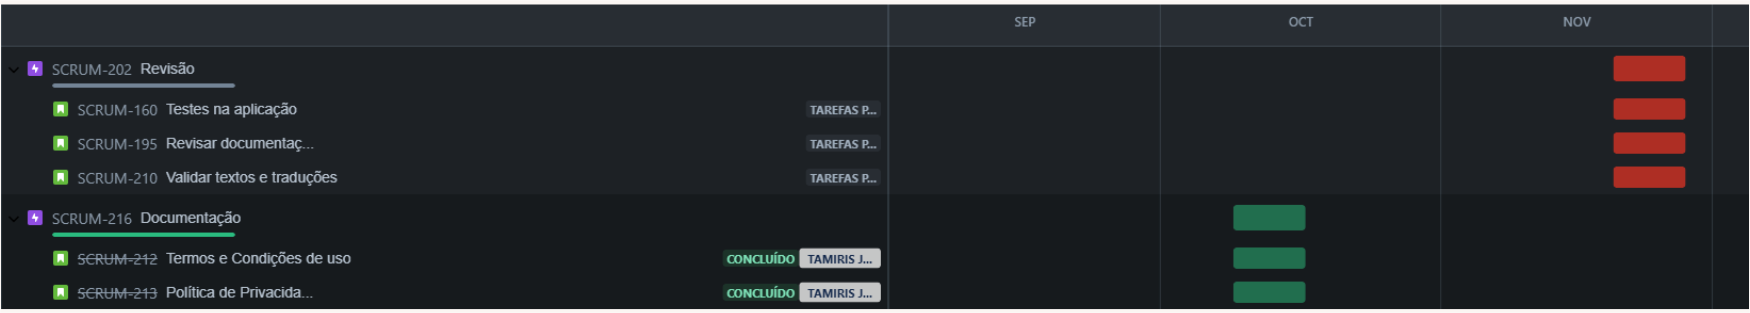
\includegraphics[width=1.0\textwidth]{images/revisao-cronograma.png}
        \caption{Cronograma definido para a revisão e documentação no segundo semestre de 2024}
        \label{fig:revisaocronograma}
    \end{figure}

O desenvolvimento do projeto e a documentação são extensos e demandam reuniões constantes para verificar o progresso e ajustar o que ainda precisa ser feito. Dessa forma, as reuniões de planejamento e verificação continuam acontecendo para garantir que a entrega final do projeto seja realizada dentro do prazo.

\chapter{TESTE DE USABILIDADE - RESULTADOS}
\label{apendice_l}

\begin{figure}[H]
    \centering
    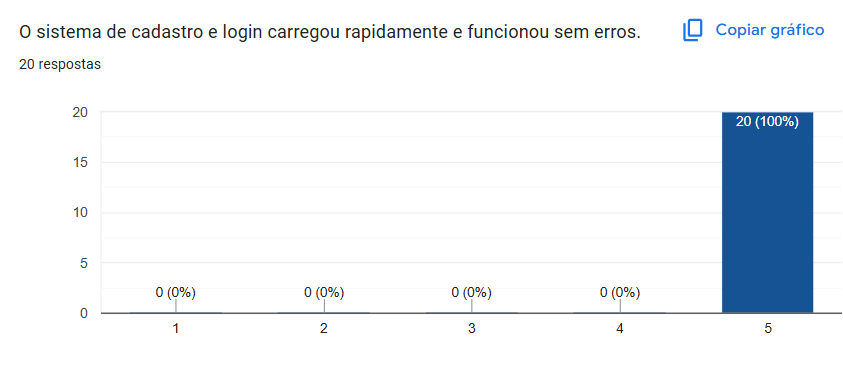
\includegraphics[width=1.0\linewidth]{images/cadastro.png}
    \caption{Processo de cadastro e login}
    \label{fig:cadastro}
\end{figure}

\begin{figure}[H]
    \centering
    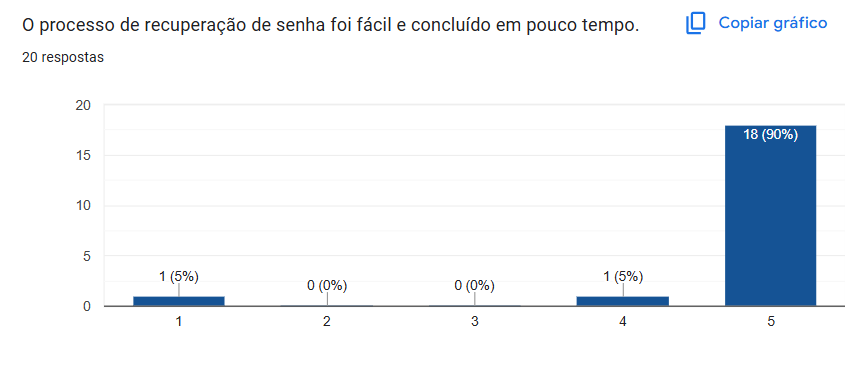
\includegraphics[width=1.0\linewidth]{images/recuperacao.png}
    \caption{Processo de recuperação de senha}
    \label{fig:senha}
\end{figure}

\begin{figure}[H]
    \centering
    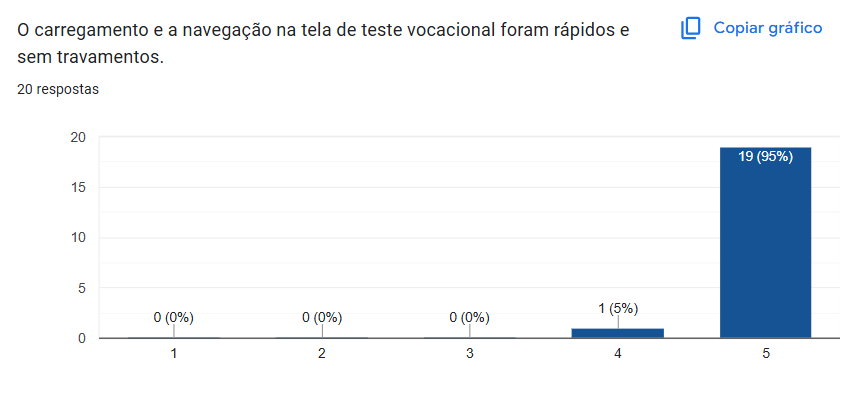
\includegraphics[width=1.0\linewidth]{images/teste.png}
    \caption{Resposta do teste vocacional}
    \label{fig:teste}
\end{figure}

\begin{figure}[H]
    \centering
    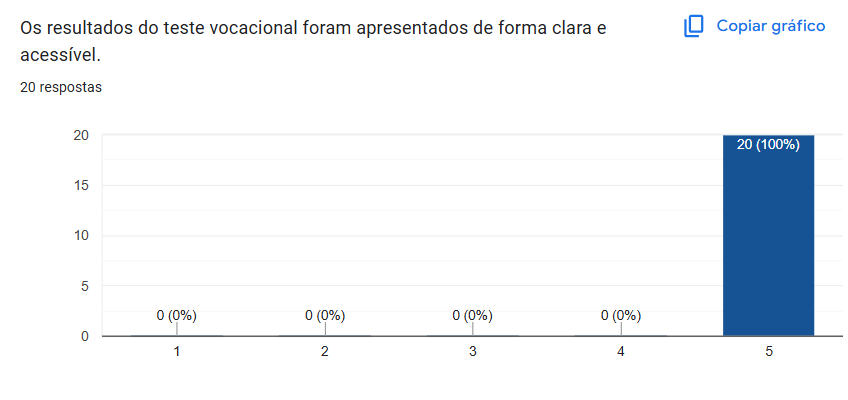
\includegraphics[width=1.0\linewidth]{images/resultado.png}
    \caption{Resultado do teste vocacional}
    \label{fig:resultado}
\end{figure}

\begin{figure}[H]
    \centering
    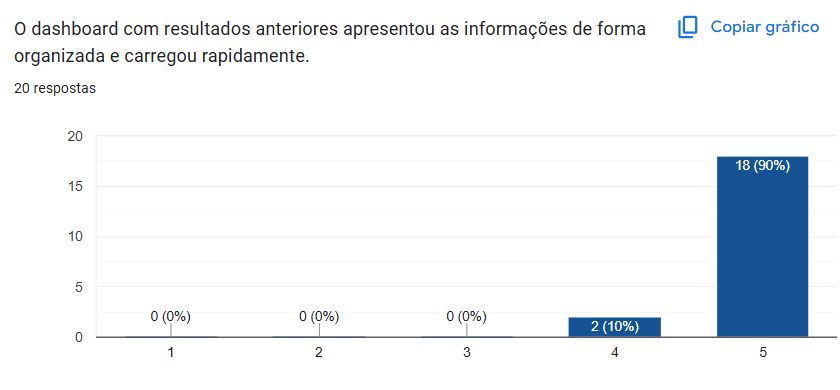
\includegraphics[width=1.0\linewidth]{images/resultadoAnterior.png}
    \caption{Dashboard}
    \label{fig:resultadoAnterior}
\end{figure}

\begin{figure}[H]
    \centering
    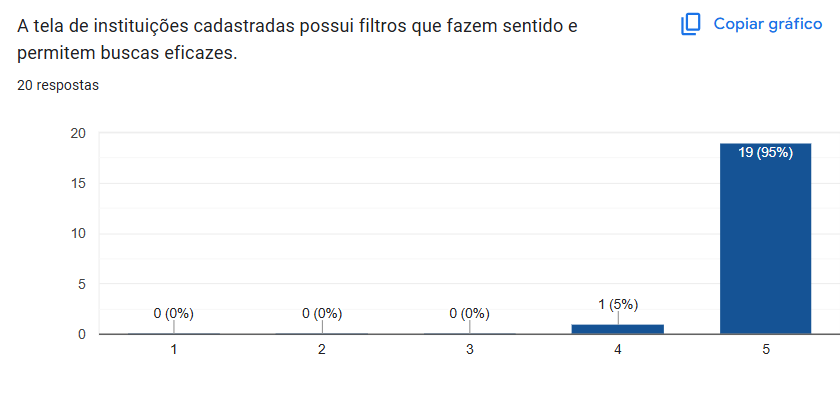
\includegraphics[width=1.0\linewidth]{images/instituicoes.png}
    \caption{Listagem de instituições}
    \label{fig:instituicoes}
\end{figure}

\begin{figure}[H]
    \centering
    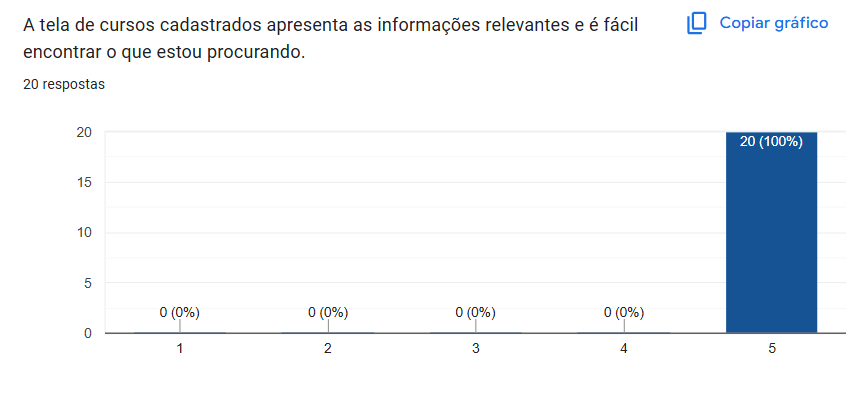
\includegraphics[width=1.0\linewidth]{images/cursosListagem.png}
    \caption{Listagem de cursos}
    \label{fig:cursos}
\end{figure}

\begin{figure}[H]
    \centering
    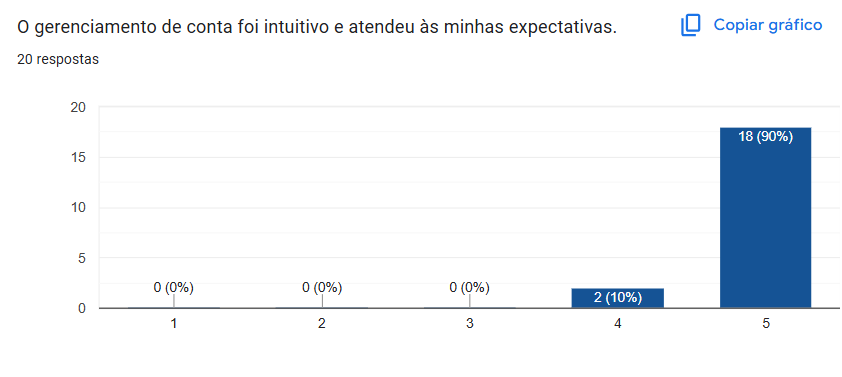
\includegraphics[width=1.0\linewidth]{images/conta.png}
    \caption{Gerenciamento de conta}
    \label{fig:conta}
\end{figure}


\begin{figure}[H]
    \centering
    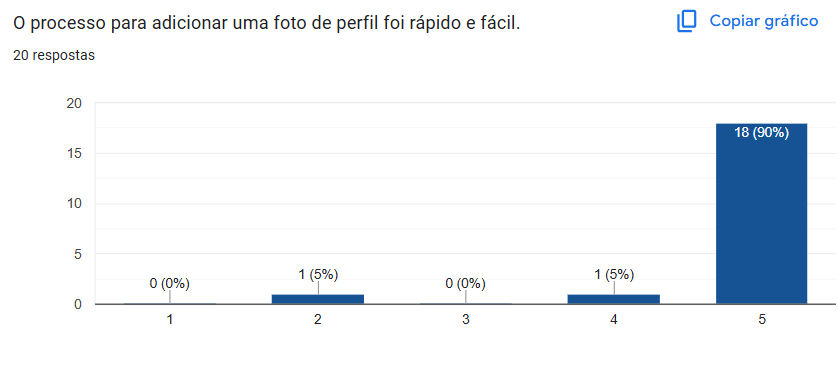
\includegraphics[width=1.0\linewidth]{images/fotoPerfil.png}
    \caption{Adição da foto de perfil}
    \label{fig:fotoPerfil}
\end{figure}

\begin{figure}[H]
    \centering
    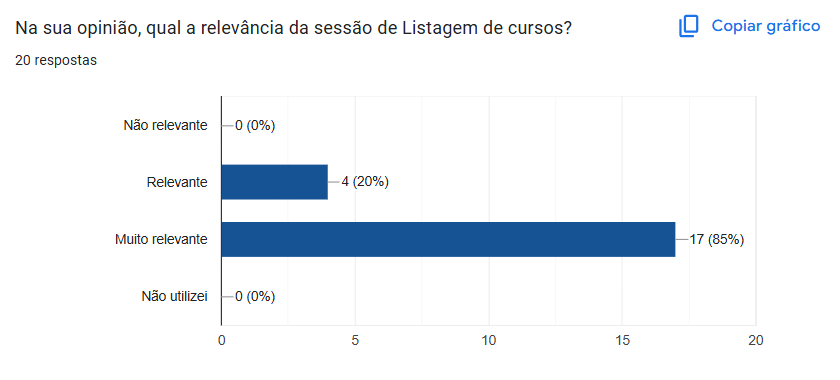
\includegraphics[width=1.0\linewidth]{images/relevanciaCursos.png}
    \caption{Relevância da tela de listagem de cursos}
    \label{fig:relevanciaCursos}
\end{figure}

\begin{figure}[H]
    \centering
    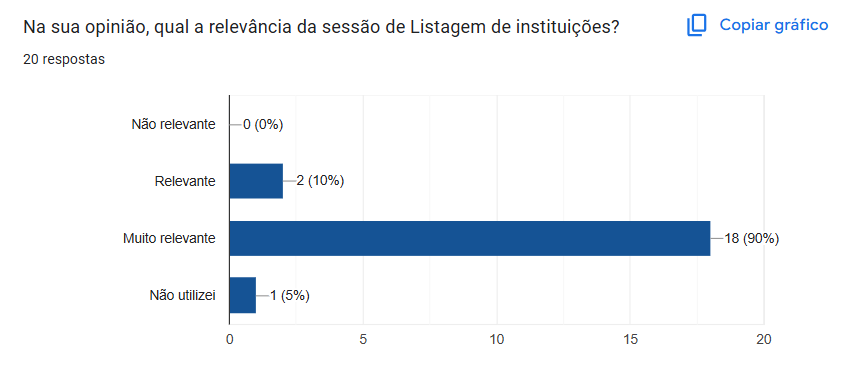
\includegraphics[width=1.0\linewidth]{images/relevanciaInstituicao.png}
    \caption{Relevância da tela de listagem de instituições}
    \label{fig:relevanciaInstituicoes}
\end{figure}

\begin{figure}[H]
    \centering
    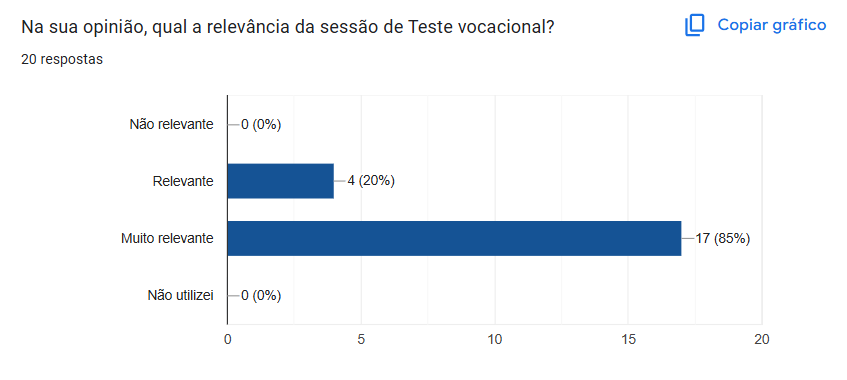
\includegraphics[width=1.0\linewidth]{images/relevanciaTeste.png}
    \caption{Relevância do teste vocacional}
    \label{fig:relevanciaTeste}
\end{figure}


\begin{figure}[H]
    \centering
    \includegraphics[width=0.85\linewidth]{images/sugestões1.png}
    \caption{Sugestões de melhoria}
    \label{fig:sugestoes}
\end{figure}


\begin{figure}[H]
    \centering
    \includegraphics[width=0.85\linewidth]{images/sugestões2.png}
    \caption{Sugestões de melhoria}
    \label{fig:sugestoes}
\end{figure}


\begin{figure}[H]
    \centering
    \includegraphics[width=0.85\linewidth]{images/sugestões3.png}
    \caption{Sugestões de melhoria}
    \label{fig:sugestoes}
\end{figure}

\chapter{Atas de Reuniões}
\label{apendice_j}

\section*{Reunião 10/03}

\subsection*{Participantes}
Beatriz Andrade, Isadora Câmara, Letícia Baião, Suanne Almeida, Tamiris Jesus.

\subsection*{Pauta}
\begin{itemize}
    \item Estudo de viabilidade do projeto, considerando o fluxo de atividades necessárias para a sua realização.
    \item Desenvolvimento e organização do documento de introdução.
    \item Divisão dos temas a serem abordados na apresentação da próxima semana.
\end{itemize}

\subsection*{Observações}
Primeira reunião realizada, marcando o início oficial do projeto. 
Decisão de cada membro gravar sua parte da apresentação para posterior edição em um vídeo a ser publicado no canal da equipe no YouTube. 

\subsection*{Ações Necessárias}
\begin{itemize}
    \item Definição da proposta da plataforma e seus objetivos.
    \item Análise das propostas para o desenvolvimento do cálculo de compatibilidade a ser utilizado no teste vocacional.
    \item Estudo de ideias para potenciais fontes de financiamento e oportunidades de parcerias.
    \item Transferência do documento de introdução para o Overleaf.
    \item Início da elaboração dos slides para a apresentação.
\end{itemize}

\subsection*{Pauta da Próxima Semana}
Para a próxima semana, ficou definido que iremos unir as partes gravadas por cada integrante para o vídeo.

\section*{Reunião 13/03}

\subsection*{Participantes}
Beatriz Andrade, Isadora Câmara, Letícia Baião, Tamiris Jesus, Suanne Almeida.

\subsection*{Pauta}
\begin{itemize}
    \item Acompanhamento da última reunião: Os vídeos de cada integrante foram agrupados em um único vídeo, o qual já foi publicado no canal do YouTube da equipe, conforme o proposto na reunião anterior. 
    \item Novos assuntos:
    \begin{itemize}
        \item Discussão sobre o algoritmo responsável pelo cálculo de compatibilidade a ser utilizado no teste vocacional.
        \item Definição de cargos para cada membro da equipe.
        \item Análise de estratégias para o controle de versão.
        \item Análise de estratégias para a documentação.
    \end{itemize}
\end{itemize}

\subsection*{Observações}
Não foi realizada uma reunião para consolidar as partes dos vídeos gravados por cada integrante em um único vídeo.
Cada membro da equipe assumiu a responsabilidade de realizar pesquisas referentes à proposta do projeto e analisar o funcionamento dos testes vocacionais em plataformas concorrentes.

\subsection*{Ações Necessárias}
\begin{itemize}
    \item Avaliação de perspectivas sobre o algoritmo a ser usado no cálculo de compatibilidade, juntamente com as suposições relacionadas às funcionalidades e ao fluxo.
    \item Análise das habilidades/afinidades individuais de cada integrante para determinar a área em que melhor se encaixa no projeto.
    \item Avaliação e decisão sobre qual método de ramificação utilizar para o controle de versão.
    \item Definição das ferramentas de documentação a serem utilizadas.
\end{itemize}

\subsection*{Pauta da Próxima Semana}
\begin{itemize}
    \item Apresentar os resultados e sugestões de aprimoramento dos testes vocacionais a serem analisados.
    \item \textit{Brainstorming} de funcionalidades para o sistema.
    \item Elaborar uma proposta de projeto para concorrer ao Prêmio Luz na Educação.
\end{itemize}

\section*{Reunião 20/03}

\subsection*{Participantes}
Beatriz Andrade, Isadora Câmara, Letícia Baião, Tamiris Jesus, Suanne Almeida.

\subsection*{Pauta}
\begin{itemize}
    \item Acompanhamento da última reunião: Cada membro da equipe cumpriu sua responsabilidade ao realizar pesquisas sobre a proposta do projeto e analisar o funcionamento dos testes vocacionais em plataformas concorrentes.
    \item Novos assuntos:
    \begin{itemize}
        \item Discussão sobre como funciona o \ac{svn} e como subiremos nossos arquivos, incluindo o compartilhamento do link do YouTube, a apresentação de slides e o documento de introdução.
        \item Análise dos testes vocacionais realizados em plataformas concorrentes.
    \end{itemize}
\end{itemize}

\subsection*{Observações}
O brainstorming de funcionalidades para o sistema e a elaboração de uma proposta de projeto para concorrer ao Prêmio Luz na Educação não foram realizados.

\subsection*{Ações Necessárias}
\begin{itemize}
    \item Cada integrante compartilhou suas experiências com os testes vocacionais, discutindo o que mais gostaram, o que menos gostaram, as vantagens e as desvantagens.
    \item Análise do que de positivo podemos extrair dos testes vocacionais estudados para aplicar em nosso projeto.
    \item Pré-seleção dos requisitos para os testes vocacionais.
\end{itemize}

\subsection*{Pauta da Próxima Semana}
\begin{itemize}
    \item Definição de requisitos, incluindo requisitos funcionais, não funcionais e regras de negócio.
    \item Brainstorming de funcionalidades para o sistema.
    \item Elaborar uma proposta de projeto para concorrer ao Prêmio Luz na Educação.
\end{itemize}

\section*{Reunião 27/03}

\subsection*{Participantes}
Beatriz Andrade, Isadora Câmara, Tamiris Jesus, Suanne Almeida.

\subsection*{Pauta}
\begin{itemize}
    \item Novos assuntos:
    \begin{itemize}
        \item Discussão sobre as funcionalidades do sistema e as entidades que serão implementadas.
        \item Discussão sobre as vantagens das tecnologias que serão utilizadas no frontend.
        \item Início da definição de requisitos, abrangendo requisitos funcionais, não funcionais e regras de negócio.
    \end{itemize}
\end{itemize}

\subsection*{Observações}
A definição dos requisitos do sistema não foi concluída e a elaboração de uma proposta de projeto para concorrer ao Prêmio Luz na Educação não foi realizada.
Foi sugerido que assistíssemos às aulas recomendadas por uma integrante do grupo sobre o uso do TypeScript em uma aplicação.

\subsection*{Ações Necessárias}
\begin{itemize}
    \item Discutimos as funcionalidades que nosso sistema terá, avaliando quais são essenciais para a fase atual e quais pretendemos implementar posteriormente.
    \item No contexto das funcionalidades, analisamos quais entidades seriam necessárias em nosso sistema.
    \item Discutimos as vantagens do React e do TypeScript, bem como as otimizações que essas tecnologias trariam para o projeto.
    \item Elaboração de um documento que contém os requisitos, abrangendo tanto os requisitos funcionais quanto os não funcionais, além das regras de negócio.
\end{itemize}

\subsection*{Pauta da Próxima Semana}
\begin{itemize}
    \item Continuação da definição de requisitos, incluindo requisitos funcionais, não funcionais e regras de negócio.
    \item Início do esboço do desenho da arquitetura da aplicação.
    \item Elaborar uma proposta de projeto para concorrer ao Prêmio Luz na Educação.
\end{itemize}

\section*{Reunião 28/03}

\subsection*{Participantes}
Beatriz Andrade, Isadora Câmara, Letícia Baião, Tamiris Jesus, Suanne Almeida.

\subsection*{Pauta}
\begin{itemize}
    \item Novos assuntos:
    \begin{itemize}
        \item Atualização para todos os membros sobre as entidades do sistema e esclarecimento de dúvidas/inseguranças referentes à implantação do sistema na Amazon Web Service.
        \item Definição de todos os elementos que precisam ser incluídos no desenho da aplicação.
        \item Elaboração da proposta e inscrição para o Prêmio Luz na Educação.
    \end{itemize}
\end{itemize}

\subsection*{Observações}
Não foi proposta uma alternativa definitiva para substituir a implantação do sistema na \textbf{Amazon Web Service}.

\subsection*{Ações Necessárias}
\begin{itemize}
    \item Discutimos os prós e contras de implantar a plataforma na \textbf{Amazon Web Service}.
    \item Dividimos as partes que devem ser escritas para elaborar a documentação do desenho da aplicação entre as integrantes.
    \item Lemos o rascunho da proposta elaborado pela integrante Tamiris e realizamos os ajustes e melhorias necessários.
    \item Lemos a documentação do Prêmio Luz na Educação e seguimos todas as etapas necessárias para a inscrição.
\end{itemize}

\subsection*{Pauta da Próxima Semana}
\begin{itemize}
    \item Cada integrante será responsável por realizar a sua parte na documentação dos desenhos da aplicação.
    \item Ficou definido que as integrantes irão estudar e avaliar outras propostas para substituir a \textbf{Amazon Web Service} como plataforma de infraestrutura.
\end{itemize}

\section*{Reunião 03/04}

\subsection*{Participantes}
Beatriz Andrade, Isadora Câmara, Letícia Baião, Tamiris Jesus, Suanne Almeida.

\subsection*{Pauta}
\begin{itemize}
    \item Novos assuntos:
    \begin{itemize}
        \item Escolha de publicar toda a documentação no GitHub.
        \item Divisão das responsabilidades de criação dos slides entre as integrantes.
        \item Ajustes de configuração no \textbf{Overleaf}.
    \end{itemize}
\end{itemize}

\subsection*{Observações}
Após análises e estudos, as integrantes ficaram em dúvida entre duas plataformas para a implantação do sistema: \textbf{Heroku} e \textbf{Railway}.

\subsection*{Ações Necessárias}
\begin{itemize}
    \item Discutimos a divisão das responsabilidades na criação dos slides entre as integrantes.
    \item Foi feita a confirmação que a configuração do \textbf{Overleaf} que devemos utilizar é aquela enviada pelo professor.
    \item Nós definimos e validamos todos os requisitos do projeto.
    \item Decidimos que, a partir de agora, vamos incluir os áudios dos vídeos de apresentação diretamente nos slides do Canva.
\end{itemize}

\subsection*{Pauta da Próxima Semana}
\begin{itemize}
    \item As integrantes assumiram o compromisso de cada uma realizar sua parte nos slides, incluindo a gravação dos áudios a serem incorporados no Canva.
    \item As integrantes realizarão um estudo comparativo entre as plataformas Heroku e Railway para decidir qual delas deve ser utilizada para a infraestrutura.
\end{itemize}

\section*{Reunião 10/04}

\subsection*{Participantes}
Beatriz Andrade, Isadora Câmara, Letícia Baião, Tamiris Jesus, Suanne Almeida.

\subsection*{Pauta}
\begin{itemize}
    \item Novos assuntos:
    \begin{itemize}
        \item Análise da Prova de Conceito.
    \end{itemize}
\end{itemize}

\subsection*{Observações}
Reunião apenas para discutir a Prova de Conceito que deverá ser entregue.

\subsection*{Ações Necessárias}
\begin{itemize}
    \item Realizamos uma reunião em que discutimos minuciosamente e dividimos todas as etapas necessárias para a conclusão bem-sucedida da Prova de Conceito.
\end{itemize}

\subsection*{Pauta da Próxima Semana}
\begin{itemize}
    \item Ficou decidido que as integrantes começarão a trabalhar na documentação e se reunirão posteriormente para planejar o desenvolvimento do sistema.
\end{itemize}

\section*{Reunião 24/04}

\subsection*{Participantes}
Beatriz Andrade, Isadora Câmara, Letícia Baião, Tamiris Jesus, Suanne Almeida.

\subsection*{Pauta}
\begin{itemize}
    \item Novos assuntos:
    \begin{itemize}
        \item Escolha do modelo de referência para o código de personalidade que servirá de base para o teste vocacional.
        \item Escolha da ferramenta de construção para o \textit{frontend}.
    \end{itemize}
\end{itemize}

\subsection*{Observações}
A reunião também serviu para alinhar todas as integrantes quanto aos estudos em andamento, tanto no desenvolvimento \textit{backend} quanto no \textit{frontend}.

\subsection*{Ações Necessárias}
\begin{itemize}
    \item Realizamos uma pesquisa para identificar modelos de referência existentes para testes vocacionais ou avaliações de personalidade.
    \item Optamos por utilizar o modelo de código de personalidade de John Holland.
    \item Debatemos sobre as ferramentas de construção para o \textit{frontend} e optamos por utilizar o Vite.
\end{itemize}

\subsection*{Pauta da Próxima Semana}
\begin{itemize}
    \item Ficou decidido que as integrantes irão se reunir para elaborar como devem prosseguir no fluxo do desenvolvimento das telas.
\end{itemize}

\section*{Reunião 28/04}

\subsection*{Participantes}
Beatriz Andrade, Isadora Câmara, Letícia Baião, Tamiris Jesus, Suanne Almeida.

\subsection*{Pauta}
\begin{itemize}
    \item Novos assuntos:
    \begin{itemize}
        \item Desenvolvimento do \textit{design} das telas que serão implementadas no fluxo do perfil do administrador.
    \end{itemize}
\end{itemize}

\subsection*{Observações}
Como esses eram protótipos de baixa fidelidade, os desenhos das telas foram feitos no Canva.

\subsection*{Ações Necessárias}
\begin{itemize}
    \item As integrantes que estavam responsáveis pelo \textit{backend} orientaram as colegas encarregadas do \textit{frontend} no desenvolvimento das telas.
    \item Optamos por utilizar o modelo de código de personalidade de John Holland.
    \item Analisamos completamente os requisitos específicos do perfil do administrador e os fluxos que as telas devem suportar.
    \item Criamos \textit{wireframes} detalhados das telas.
\end{itemize}

\subsection*{Pauta da Próxima Semana}
\begin{itemize}
    \item Ficou decidido que as integrantes se reunirão para alinhar o desenvolvimento das telas.
\end{itemize}

\section*{Reunião 01/05}

\subsection*{Participantes}
Beatriz Andrade, Isadora Câmara, Letícia Baião, Tamiris Jesus, Suanne Almeida.

\subsection*{Pauta}
\begin{itemize}
    \item Novos assuntos:
    \begin{itemize}
        \item Discussão sobre o desenvolvimento das telas conforme os \textit{wireframes}.
        \item Atualização do progresso individual de cada integrante no projeto.
    \end{itemize}
\end{itemize}

\subsection*{Observações}
As telas estão sendo desenvolvidas de acordo com os protótipos de baixa fidelidade criados anteriormente.
Cada integrante compartilhou seu progresso e contribuições até o momento.

\subsection*{Ações Necessárias}
\begin{itemize}
    \item Implementação das alterações nos \textit{wireframes} conforme discutido.
    \item Continuação do desenvolvimento das telas com base nos requisitos estabelecidos.
\end{itemize}

\section*{Reunião 08/05}

\subsection*{Participantes}
Beatriz Andrade, Isadora Câmara, Letícia Baião, Tamiris Jesus, Suanne Almeida.

\subsection*{Pauta}
\begin{itemize}
    \item Novos assuntos:
    \begin{itemize}
        \item Discussão sobre os \textit{feedbacks} recebidos durante a apresentação.
        \item Planejamento dos próximos passos para a próxima entrega.
    \end{itemize}
\end{itemize}

\subsection*{Observações}
Como esses eram protótipos de baixa fidelidade, os desenhos das telas foram feitos no Canva.

\subsection*{Ações Necessárias}
\begin{itemize}
    \item O projeto foi apresentado e bem recebido pelo professor orientador.
    \item Foram discutidas melhorias sugeridas pelos \textit{feedbacks} recebidos.
\end{itemize}

\subsection*{Pauta da Próxima Semana}
\begin{itemize}
    \item Ficou decidido que as integrantes se reunirão para alinhar o desenvolvimento da próxima entrega.
\end{itemize}

\section*{Reunião 11/09}

\subsection*{Participantes}
Beatriz Andrade, Isadora Câmara, Letícia Baião, Tamiris Jesus, Suanne Almeida.

\subsection*{Pauta}
\begin{itemize}
    \item Novos assuntos:
    \begin{itemize}
        \item Discussão sobre o cronograma do segundo semestre.
        \item Ajustes das tarefas no Jira.
    \end{itemize}
\end{itemize}

\subsection*{Observações}
 Definimos as datas de entrega de cada tarefa que deve ser desenvolvida do projeto.

\subsection*{Ações Necessárias}
\begin{itemize}
    \item Divisão de tarefas.
    \item Desenvolvimento do projeto.
    \item Ajustes das datas e tarefas no Jira. 
\end{itemize}

\section*{Reunião 18/09}

\subsection*{Participantes}
Beatriz Andrade, Isadora Câmara, Letícia Baião, Tamiris Jesus, Suanne Almeida.

\subsection*{Pauta}
\begin{itemize}
    \item Novos assuntos:
    \begin{itemize}
        \item Andamento do desenvolvimento.
        \item Prototipação de telas.
    \end{itemize}
\end{itemize}

\subsection*{Observações}
 Atualizamos o grupo sobre o andamento do projeto por cada integrante

\subsection*{Ações Necessárias}
\begin{itemize}
    \item Cadastro de Instituições em nossa base de dados.
    \item Prototipação de telas.
    \item Ilustrações do site.
\end{itemize}

\section*{Reunião 25/09}

\subsection*{Participantes}
Beatriz Andrade, Isadora Câmara, Letícia Baião, Tamiris Jesus, Suanne Almeida.

\subsection*{Pauta}
\begin{itemize}
    \item Novos assuntos:
    \begin{itemize}
        \item Mapeamento de cursos de graduação, técnicos e políticas públicas.
        \item Prototipação de telas.
    \end{itemize}
\end{itemize}

\subsection*{Observações}
 Discussões e definições sobre o mapeamento de dados e refatoração de telas.

\subsection*{Ações Necessárias}
\begin{itemize}
    \item Mapeamento de cursos técnicos e superiores no banco.
    \item Refatoração no \textit{front-end}.
    \item Ilustrações do site.
\end{itemize}

\section*{Reunião 02/10}

\subsection*{Participantes}
Beatriz Andrade, Isadora Câmara, Letícia Baião, Tamiris Jesus, Suanne Almeida.

\subsection*{Pauta}
\begin{itemize}
    \item Novos assuntos:
    \begin{itemize}
        \item Ilustrações da Home Page.
        \item Refatoração de telas.
        \item Mapeamento de políticas públicas, e cadastros de cursos de graduação.
    \end{itemize}
\end{itemize}

\subsection*{Observações}
 Alinhamento das ilustrações da home page, refatoração de telas e mapeamento de dados.

\subsection*{Ações Necessárias}
\begin{itemize}
    \item Mapeamento de cursos técnicos e superiores no banco.
    \item Refatoração no \textit{front-end}.
    \item Ilustrações do site.
\end{itemize}

\section*{Reunião 09/10}

\subsection*{Participantes}
Beatriz Andrade, Isadora Câmara, Letícia Baião, Tamiris Jesus, Suanne Almeida.

\subsection*{Pauta}
\begin{itemize}
    \item Novos assuntos:
    \begin{itemize}
        \item Preparação e refinamento das ilustrações.
        \item Cadastro de políticas públicas e cursos de graduação.
    \end{itemize}
\end{itemize}

\subsection*{Observações}
Foco na parte 2 do refatoramento da tela de resultado, de gerenciamento e a continuação da tela de cadastro de estudante. 

\subsection*{Ações Necessárias}
\begin{itemize}
    \item Refatoração de telas.
    \item Cadastro de políticas públicas e cursos de graduação.
    \item Preparação e refinamento das ilustrações.
\end{itemize}

\section*{Reunião 16/10}

\subsection*{Participantes}
Beatriz Andrade, Isadora Câmara, Letícia Baião, Tamiris Jesus, Suanne Almeida.

\subsection*{Pauta}
\begin{itemize}
    \item Novos assuntos:
    \begin{itemize}
        \item Ajustes na estrutura para os tipos de instituição.
        \item Cadastro na base de dados.
    \end{itemize}
\end{itemize}

\subsection*{Observações}
Ajustes e adequações na estrutura do sistema para atender cursos técnicos e de graduação.

\subsection*{Ações Necessárias}
\begin{itemize}
    \item Ajustes na estrutura para os tipos de instituição.
    \item Refatoração de telas
\end{itemize}

\section*{Reunião 23/10}

\subsection*{Participantes}
Beatriz Andrade, Isadora Câmara, Letícia Baião, Tamiris Jesus, Suanne Almeida.

\subsection*{Pauta}
\begin{itemize}
    \item Novos assuntos:
    \begin{itemize}
        \item Continuidade no refatoramento de telas com definições entre o grupo.
    \end{itemize}
\end{itemize}

\subsection*{Observações}
Ajustes e definicções do grupo sobre a refatoração das telas.

\subsection*{Ações Necessárias}
\begin{itemize}
    \item Refatoração de telas
\end{itemize}

\section*{Reunião 30/10}

\subsection*{Participantes}
Beatriz Andrade, Isadora Câmara, Letícia Baião, Tamiris Jesus, Suanne Almeida.

\subsection*{Pauta}
\begin{itemize}
    \item Novos assuntos:
    \begin{itemize}
        \item Continuidade no refatoramento de telas.
        \item Continuidade no cadastro de dados na base.
    \end{itemize}
\end{itemize}

\subsection*{Observações}
Alinhamento entre o grupo sobre as atividades de cada integrante.

\subsection*{Ações Necessárias}
\begin{itemize}
    \item Continuidade nas atividades ja exercidas.
\end{itemize}

\section*{Reunião 06/11}

\subsection*{Participantes}
Beatriz Andrade, Isadora Câmara, Letícia Baião, Tamiris Jesus, Suanne Almeida.

\subsection*{Pauta}
\begin{itemize}
    \item Novos assuntos:
    \begin{itemize}
        \item Alinhamento no inicio do último mês de desenvolvimento.
        \item Ideias de brindes.
        \item Alinhamento do andamento das tarefas de cada integrante.
    \end{itemize}
\end{itemize}

\subsection*{Observações}
Alinhamento entre o grupo sobre as atividades de cada integrante.

\subsection*{Ações Necessárias}
\begin{itemize}
    \item Continuidade nas atividades ja exercidas.
    \item Preparação e compra dos brindes.
\end{itemize}

\section*{Reunião 13/11}

\subsection*{Participantes}
Beatriz Andrade, Isadora Câmara, Letícia Baião, Tamiris Jesus, Suanne Almeida.

\subsection*{Pauta}
\begin{itemize}
    \item Novos assuntos:
    \begin{itemize}
        \item Validação dos ajustes do documento com o professor.
        \item Alinhamento entre o grupo das tarefas prontas.
        \item Ajustes na documentação e no \textit{front-end}.
    \end{itemize}
\end{itemize}

\subsection*{Observações}
Estudo e validação do documento em busca de alterações necessárias.

\subsection*{Ações Necessárias}
\begin{itemize}
    \item Ajustes na documentação, e no \textit{front-end}.
\end{itemize}

\chapter{Blog}
\label{apendice_k}
\subsection*{Primeira Publicação do Blog}
\begin{figure}[H]
    \centering
    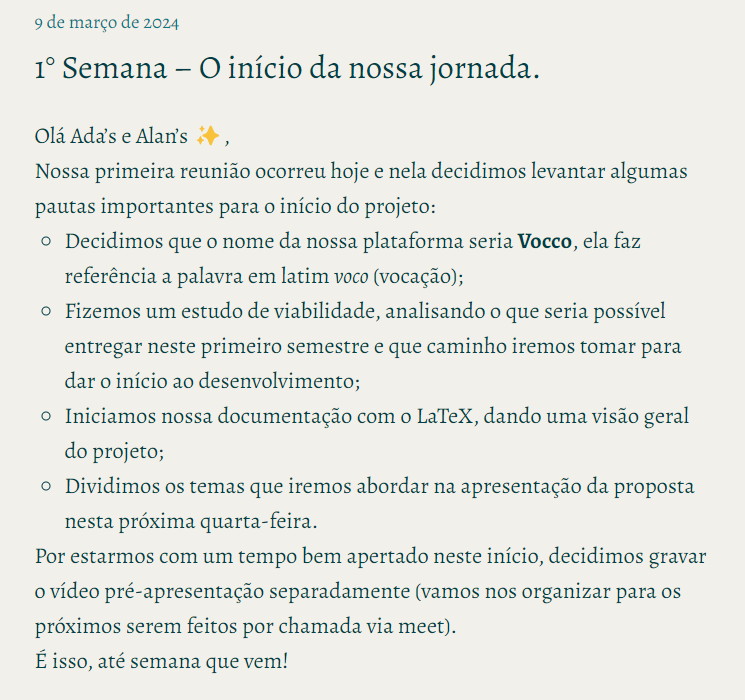
\includegraphics[width=1.0\linewidth]{images/Post1.png}
    \caption{Primeira Publicação do Blog}
    \label{fig:primeira}
\end{figure}

\subsection*{Segunda Publicação do Blog}
\begin{figure}[H]
    \centering
    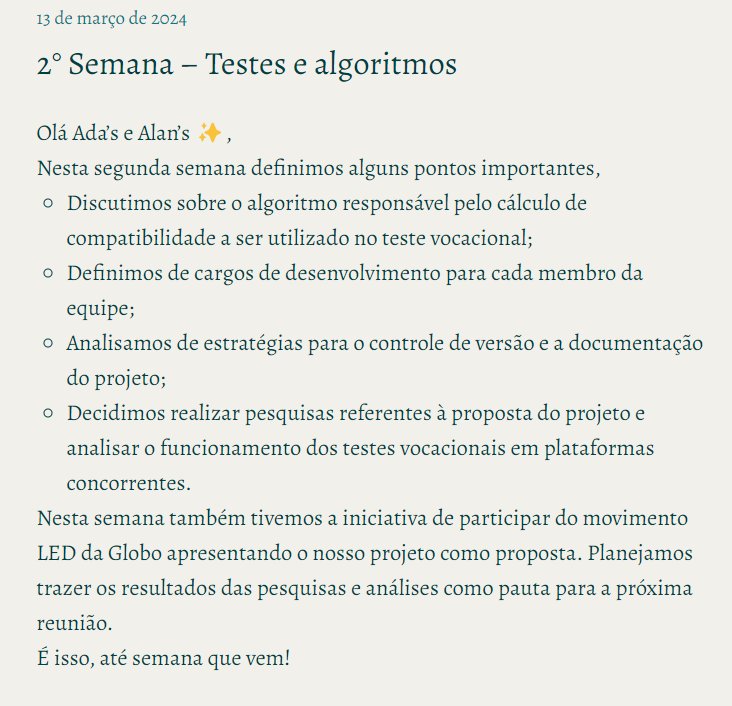
\includegraphics[width=1.0\linewidth]{images/Post2.png}
    \caption{Segunda Publicação do Blog}
    \label{fig:segunda}
\end{figure}

\subsection*{Terceira Publicação do Blog}
\begin{figure}[H]
    \centering
    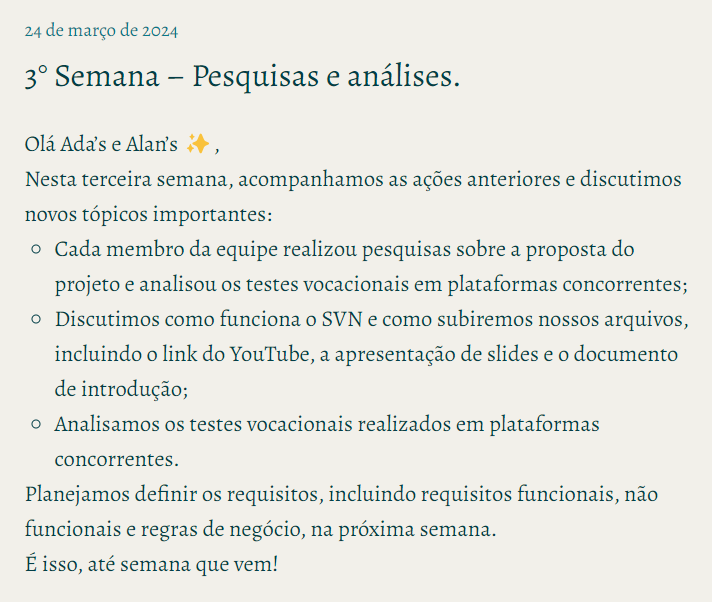
\includegraphics[width=1.0\linewidth]{images/Post3.png}
    \caption{Terceira Publicação do Blog}
    \label{fig:terceira}
\end{figure}

\subsection*{Quarta Publicação do Blog}
\begin{figure}[H]
    \centering
    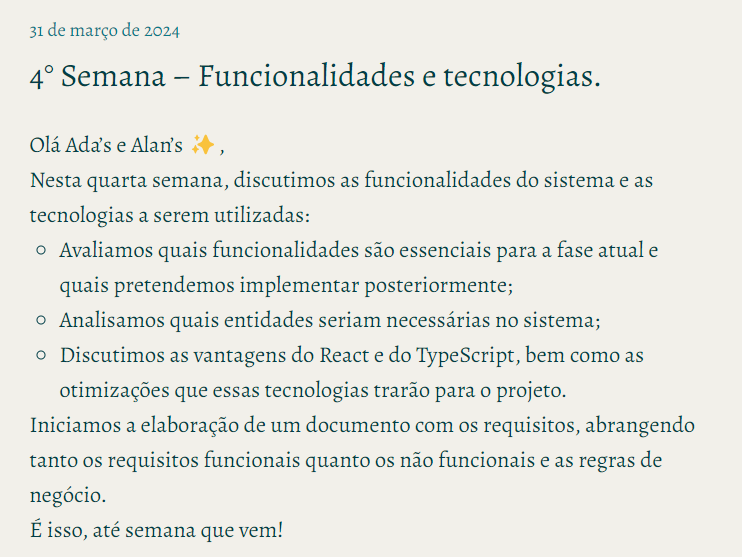
\includegraphics[width=1.0\linewidth]{images/Post4.png}
    \caption{Quarta Publicação do Blog}
    \label{fig:quarta}
\end{figure}

\subsection*{Quinta Publicação do Blog}
\begin{figure}[H]
    \centering
    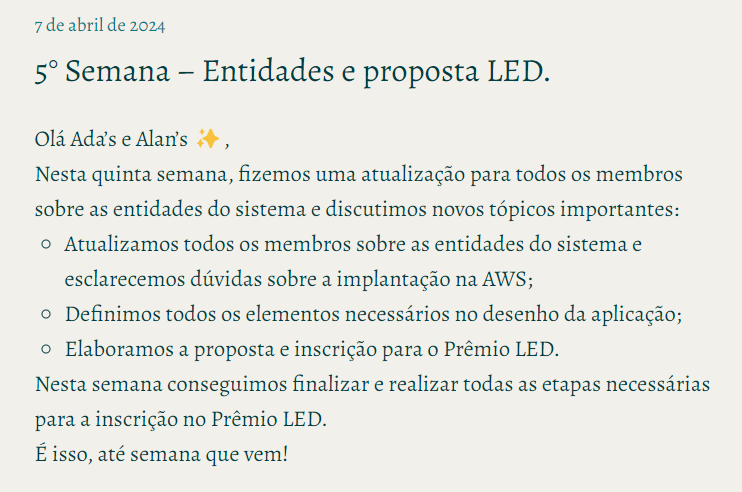
\includegraphics[width=1.0\linewidth]{images/Post5.png}
    \caption{Quinta Publicação do Blog}
    \label{fig:quinta}
\end{figure}

\subsection*{Sexta Publicação do Blog}
\begin{figure}[H]
    \centering
    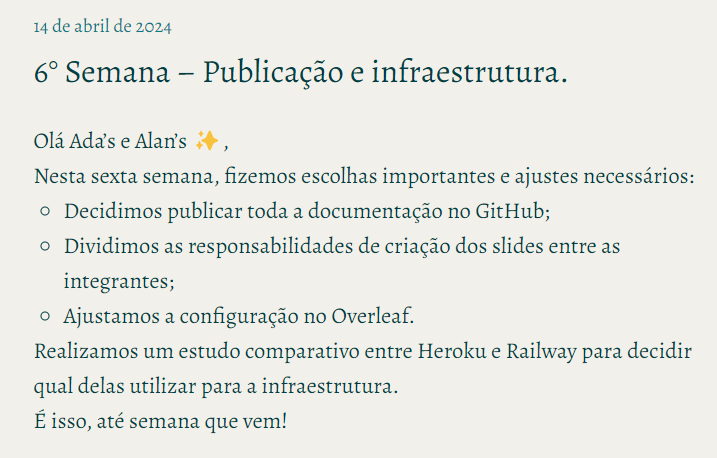
\includegraphics[width=1.0\linewidth]{images/Post6.png}
    \caption{Sexta Publicação do Blog}
    \label{fig:sexta}
\end{figure}

\subsection*{Sétima Publicação do Blog}
\begin{figure}[H]
    \centering
    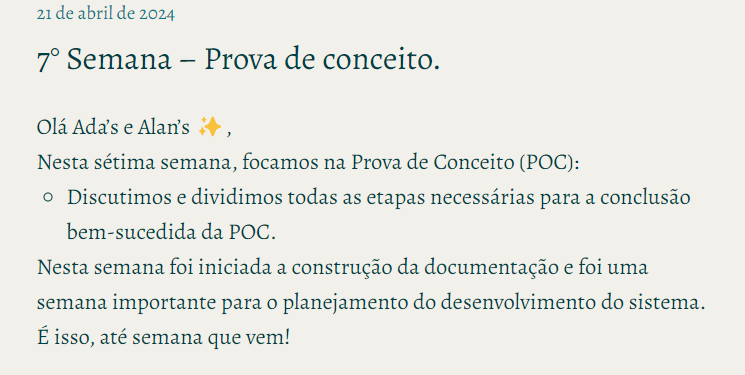
\includegraphics[width=1.0\linewidth]{images/Post7.png}
    \caption{Sétima Publicação do Blog}
    \label{fig:setima}
\end{figure}

\subsection*{Oitava Publicação do Blog}
\begin{figure}[H]
    \centering
    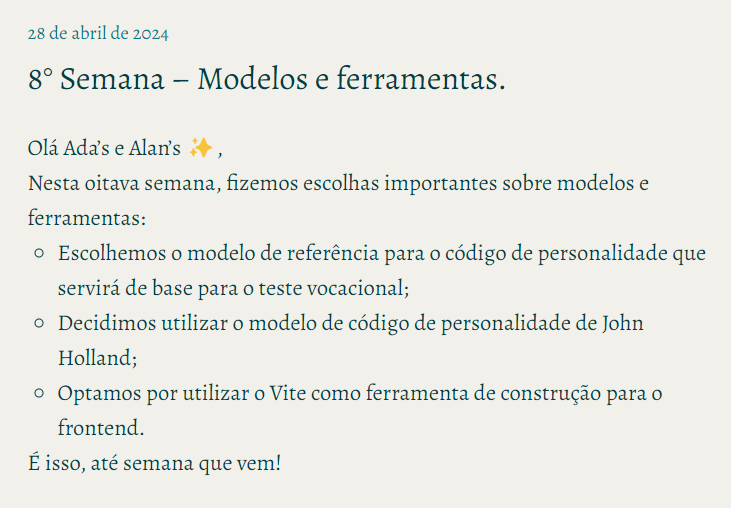
\includegraphics[width=1.0\linewidth]{images/Post8.png}
    \caption{Oitava Publicação do Blog}
    \label{fig:oitava}
\end{figure}

\subsection*{Nona Publicação do Blog}
\begin{figure}[H]
    \centering
    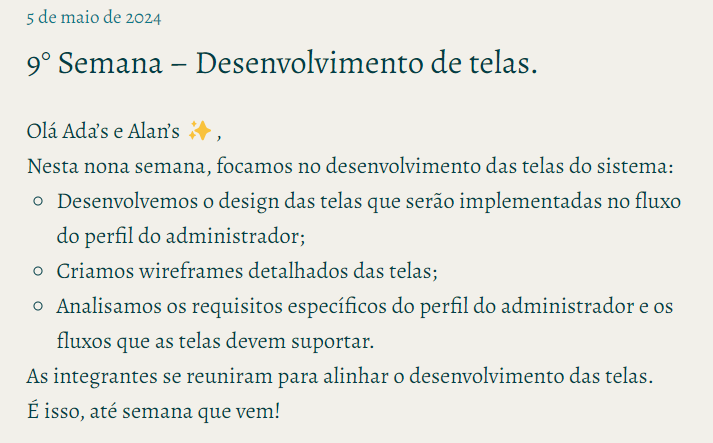
\includegraphics[width=1.0\linewidth]{images/Post9.png}
    \caption{Nona Publicação do Blog}
    \label{fig:nona}
\end{figure}

\subsection*{Décima Publicação do Blog}
\begin{figure}[H]
    \centering
    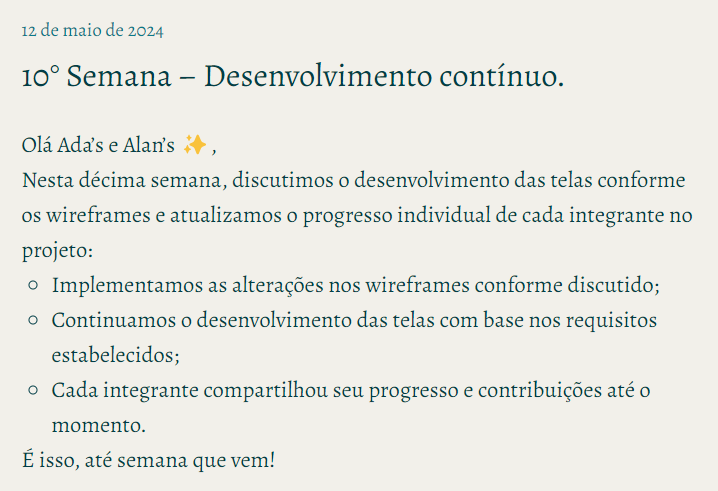
\includegraphics[width=1.0\linewidth]{images/Post10.png}
    \caption{Décima Publicação do Blog}
    \label{fig:decima}
\end{figure}

\subsection*{Décima Primeira Publicação do Blog}
\begin{figure}[H]
    \centering
    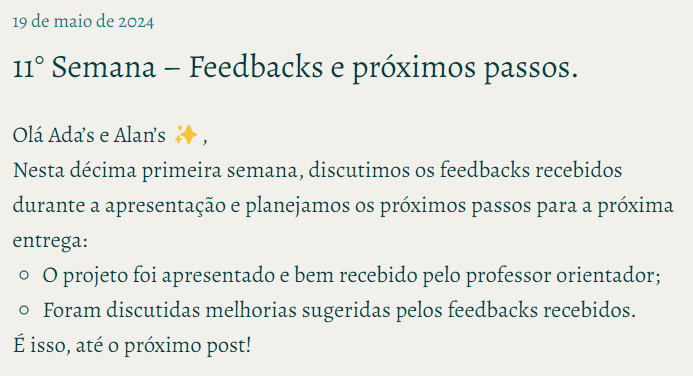
\includegraphics[width=1.0\linewidth]{images/Post11.png}
    \caption{Décima Primeira Publicação do Blog}
    \label{fig:decima primeira}
\end{figure}

\subsection*{Décima Segunda Publicação do Blog}
\begin{figure}[H]
    \centering
    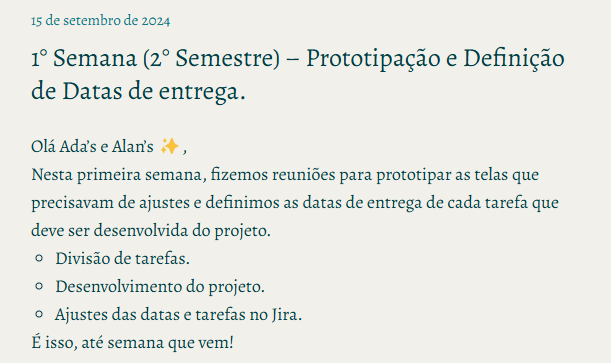
\includegraphics[width=1.0\linewidth]{images/post12.png}
    \caption{Décima Segunda Publicação do Blog}
    \label{fig:decima primeira}
\end{figure}

\subsection*{Décima Terceira Publicação do Blog}
\begin{figure}[H]
    \centering
    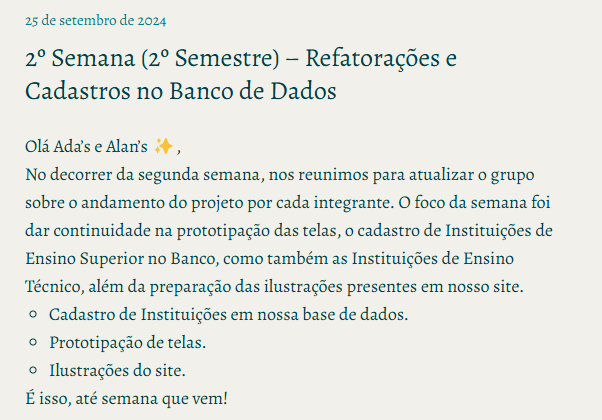
\includegraphics[width=1.0\linewidth]{images/post13.png}
    \caption{Décima Terceira Publicação do Blog}
    \label{fig:decima primeira}
\end{figure}

\subsection*{Décima Quarta Publicação do Blog}
\begin{figure}[H]
    \centering
    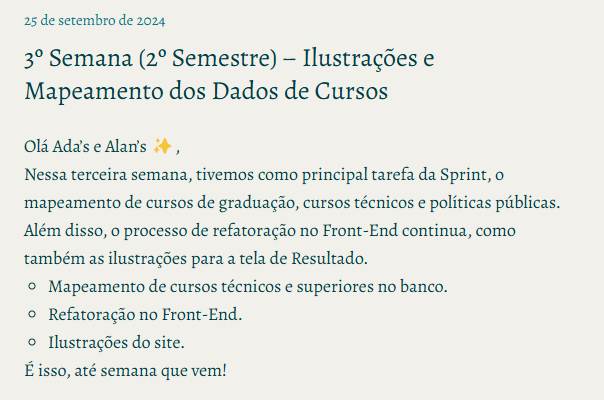
\includegraphics[width=1.0\linewidth]{images/post14.png}
    \caption{Décima Quarta Publicação do Blog}
    \label{fig:decima primeira}
\end{figure}

\subsection*{Décima Quinta Publicação do Blog}
\begin{figure}[H]
    \centering
    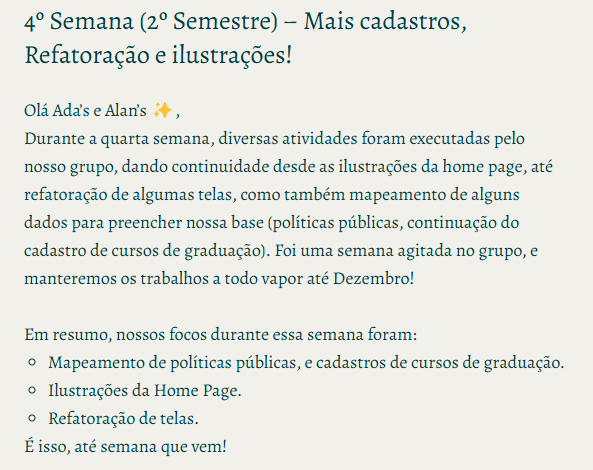
\includegraphics[width=1.0\linewidth]{images/post15.png}
    \caption{Décima Quinta Publicação do Blog}
    \label{fig:decima primeira}
\end{figure}

\subsection*{Décima Sexta Publicação do Blog}
\begin{figure}[H]
    \centering
    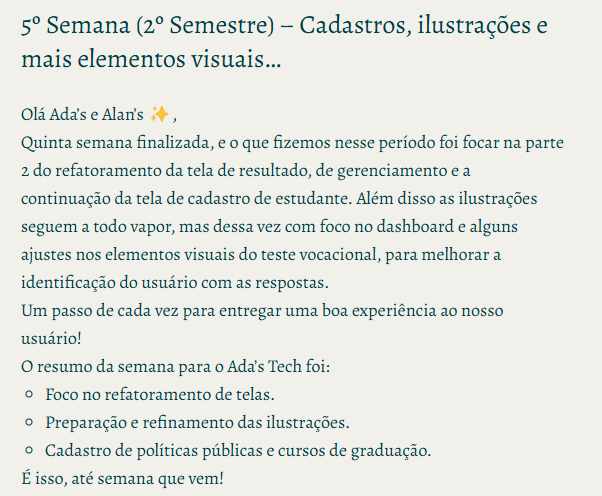
\includegraphics[width=1.0\linewidth]{images/post16.png}
    \caption{Décima Sexta Publicação do Blog}
    \label{fig:decima primeira}
\end{figure}

\subsection*{Décima Sétima Publicação do Blog}
\begin{figure}[H]
    \centering
    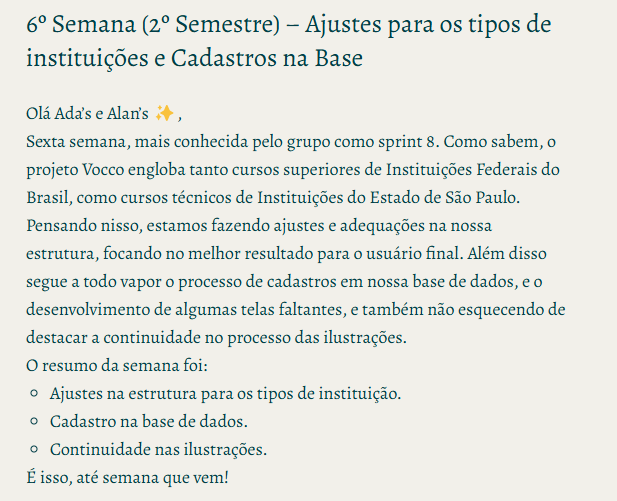
\includegraphics[width=1.0\linewidth]{images/post17.png}
    \caption{Décima Sétima Publicação do Blog}
    \label{fig:decima primeira}
\end{figure}

\subsection*{Décima Oitava Publicação do Blog}
\begin{figure}[H]
    \centering
    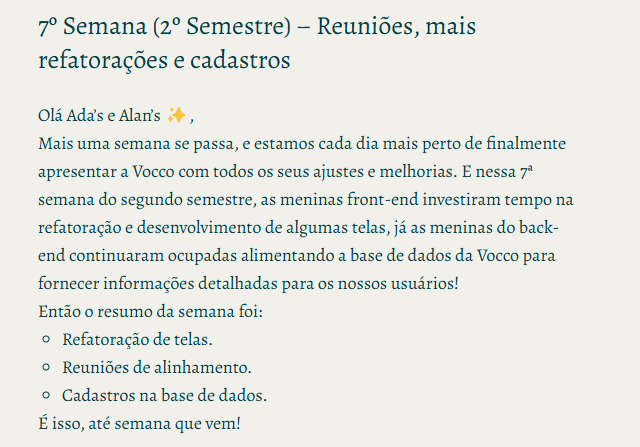
\includegraphics[width=1.0\linewidth]{images/post18.png}
    \caption{Décima Oitava Publicação do Blog}
    \label{fig:decima primeira}
\end{figure}

\subsection*{Décima Nona Publicação do Blog}
\begin{figure}[H]
    \centering
    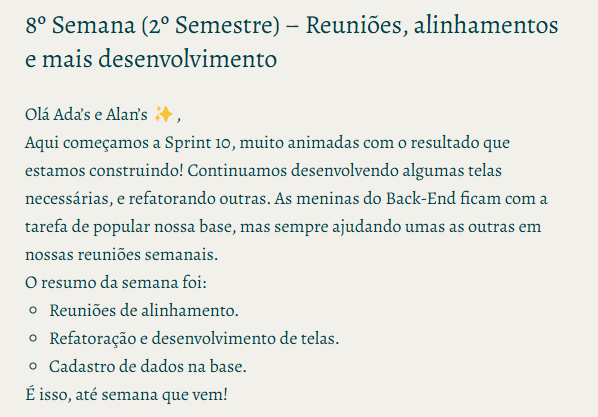
\includegraphics[width=1.0\linewidth]{images/post19.png}
    \caption{Décima Nona Publicação do Blog}
    \label{fig:decima primeira}
\end{figure}

\subsection*{Vigésima Publicação do Blog}
\begin{figure}[H]
    \centering
    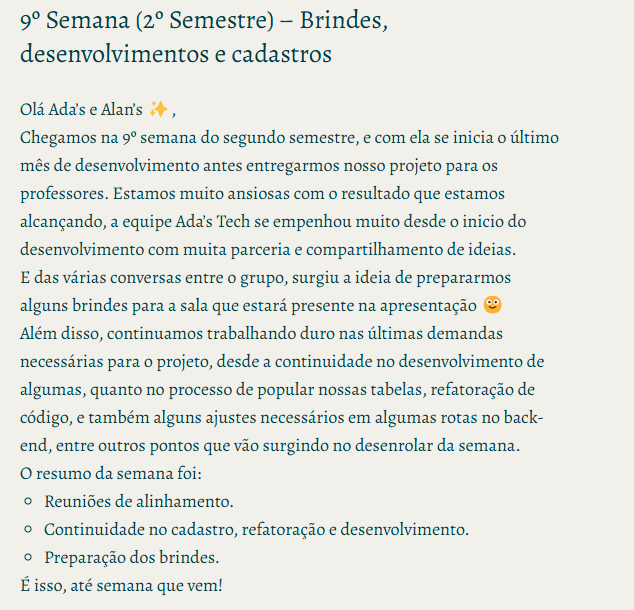
\includegraphics[width=1.0\linewidth]{images/post20.png}
    \caption{Vigésima Publicação do Blog}
    \label{fig:decima primeira}
\end{figure}

\subsection*{Vigésima Primeira Publicação do Blog}
\begin{figure}[H]
    \centering
    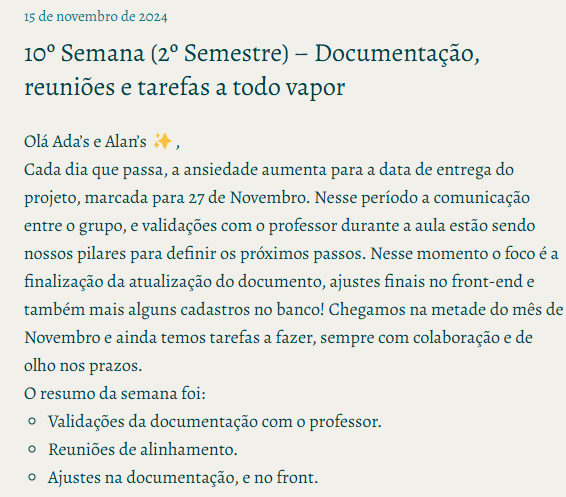
\includegraphics[width=1.0\linewidth]{images/post21.png}
    \caption{Vigésima Primeira Publicação do Blog}
    \label{fig:decima primeira}
\end{figure}




% ----------------------------------------------------------
% \chapter{Nullam elementum urna vel imperdiet sodales elit ipsum pharetra ligula
% ac pretium ante justo a nulla curabitur tristique arcu eu metus}
% % ----------------------------------------------------------
% \lipsum[3-5]

\end{apendicesenv}
% ---
